\documentclass[11pt,a4paper,oneside]{book}
%-- coding: UTF-8 --
\usepackage[UTF8]{ctex}
\usepackage{fontspec}
\usepackage{xeCJK}%文字体的设置
\newcommand{\canger}{\CJKfontspec{TsangerJinKai03}}
\setmainfont{TsangerJinKai03} %设置全文字体
\setsansfont{TsangerJinKai03}
\setCJKmainfont{TsangerJinKai03}
\setCJKsansfont{TsangerJinKai03} 
\defaultfontfeatures{Mapping=tex-text}
\usepackage{xunicode}%防止pdf乱码
%\usepackage{ccmap}%
\usepackage{multicol}%分栏 %\begin{multicols}{2} %\end{multicols}
\usepackage{xltxtra}
\usepackage{amsmath}
\usepackage{amsfonts}
\usepackage{amssymb}
\usepackage{graphicx}
\usepackage{amsthm}
\usepackage{array}
\usepackage{float}   %{H}
\usepackage{booktabs}  %\toprule[1.5pt]
\setcounter{secnumdepth}{4}
\usepackage{indentfirst} %首行缩进
\usepackage{tcolorbox} %彩色框框
\usepackage{graphicx}  %图片并排
\usepackage{subfigure} %图片并排
\usepackage{graphicx} %插入jpg
\usepackage[toc]{multitoc} %双列目录
\setcounter{secnumdepth}{4}		%增加编号深度
\setcounter{tocdepth}{4}		%增加目录深度
\usepackage{hyperref}     %生成pdf书签
\hypersetup{hidelinks,
	colorlinks=true,
	allcolors=black,
	pdfstartview=Fit,
	breaklinks=true
}       %去掉目录的红色框框
%===================%插入代码需要的控制
\usepackage{listings}
\usepackage{xcolor}
\setmonofont{Consolas}%字体
\lstset{%
	%numbers=left,
	%numberstyle=\tt\tiny,%
	showstringspaces=false,
	showspaces=false,%
	tabsize=4,%
	frame=lines,%
	basicstyle=\tt\small,%
	keywordstyle=\color{ blue!70}\bfseries,%
	identifierstyle=,%
	commentstyle=\color{red!50!green!50!blue!50},%\itshape,%
	stringstyle=\color{black},%
	breaklines=true
}
%===================%
\usepackage[left=2cm,right=2cm,top=2cm,bottom=2cm]{geometry}
\newtheorem{theorem}{定理}
\newtheorem{definition}{定义}
\newtheorem{e}{例}
\title{\Huge Beautiful Visualization with R}
\author{zy}
\date{\today}

\begin{document}
\maketitle
\tableofcontents  %目录
\chapter{R语言编程与绘图基础}
\section{编程基础}
\subsection{数据类型}

\begin{lstlisting}[language=r]
> a <- -1
> is.numeric(a)
[1] TRUE

> b <- "peter"
> nchar(b)
[1] 5

> c <- as.Date("2021-3-17")
> class(c)
[1] "Date"

#POSIXct(同时存储日期与时间)
> d <- as.POSIXct("2021-06-12 17:32")
> class(d)
[1] "POSIXct" "POSIXt" 

> e <- TRUE
> f <- FALSE
\end{lstlisting}

进一步提取日期型数据的年月周等数据信息.使用as.numeric函数或者as.integer函数将日期型数据转换成数值型,其中strftime(x,format="")函数可以定义日期型数据的格式.
	

\begin{lstlisting}[language=r]
> (c_year <- as.integer(strftime(c,'%Y')))
[1] 2021
> (c_month <- as.integer(strftime(c,'%m')))
[1] 3
> (c_week <- as.integer(strftime(c,'%W')))
[1] 11
\end{lstlisting}


\subsection{数据结构}
\subsubsection{向量}
\begin{lstlisting}[language=r]
> 2:6
[1] 2 3 4 5 6

> seq(2,3,by=0.5)
[1] 2.0 2.5 3.0

> rep(2:3,times=3)
[1] 2 3 2 3 2 3
> rep(2:4,times=3)
[1] 2 3 4 2 3 4 2 3 4
> rep(1:3,each=4)
[1] 1 1 1 1 2 2 2 2 3 3 3 3

> rnorm(3,mean=1,sd=2)
[1] 2.5404507 0.2442733 1.8078082
> runif(3,min=2,max=3)
[1] 2.795074 2.823721 2.498441

> sample(c("A","B","C"),4,replace = TRUE)
[1] "B" "A" "C" "A"
\end{lstlisting}

向量的处理:

1.排序
\begin{lstlisting}[language=r]
> v <- c(1,2,3,4,1,2,8)
> order <- sort(v,index.return=TRUE,decreasing = TRUE)
> order
$x
[1] 8 4 3 2 2 1 1 #排序

$ix
[1] 7 4 3 2 6 1 5 #排序的索引(index.return=TRUE)
\end{lstlisting}

2.向量的唯一值

unique返回一个删除了重复元素或行的向量,数据框或数组
\begin{lstlisting}[language=r]
> v2 <- c("perter","tim","pat","jack","tim","pat")
> uni <- unique(v2)
> uni
[1] "perter" "tim"    "pat"    "jack"  
\end{lstlisting}

3.连续向量的离散化

数据离散化最简单的方法就是使用cut函数自定义离散区间
\begin{lstlisting}[language=r]
> cvec <- cut(nvec,breaks = c(0,3,6,9,11),labels = c("0~3","3~6","6~9",">9"))
> cvec
[1] >9  3~6 3~6 6~9 3~6 0~3 3~6 6~9 6~9 3~6
Levels: 0~3 3~6 6~9 >9
\end{lstlisting}

\subsubsection{因子}
1.因子的创建
\begin{lstlisting}[language=r]
> cut <- c("Fair","Good","Ideal","Premium","Very Good")
> cut_factor <- as.factor(cut)
> cut_factor
[1] Fair      Good      Ideal     Premium   Very Good
Levels: Fair Good Ideal Premium Very Good
\end{lstlisting}

2.水平的更改
\begin{lstlisting}[language=r]
> cut_factor2 <- factor(x=c("Fair","Good","Ideal","Premium","Very Good"),
+                       levels = c("Premium","Good","Ideal","Fair","Very Good"),
+                       ordered = TRUE)
> cut_factor2
[1] Fair      Good      Ideal     Premium   Very Good
Levels: Premium < Good < Ideal < Fair < Very Good
\end{lstlisting}

3.类型的转换
\begin{lstlisting}[language=r]
> num_factor <- factor(x=c(1,3,5,2),levels=c(5,3,2,1),ordered=TRUE)
> num_factor
[1] 1 3 5 2
Levels: 5 < 3 < 2 < 1
> num_vector1 <- as.numeric(as.character(num_factor))
> num_vector1
[1] 1 3 5 2
> num_vector2 <- as.numeric(num_factor)
> num_vector2
[1] 4 2 1 3
\end{lstlisting}

\subsubsection{数据框}

获取数据框的行数列数维数:nrow(),ncol(),dim()

获取数据框的列名行名:names(),rownames(),colnames()

1.空数据框的创建

创建一个名为df,包括两个变量(numeric和character)
\begin{lstlisting}[language=r]
> df <- data.frame(a=numeric(),b=character(),stringsAsFactors = FALSE)
\end{lstlisting}

或者可以先使用矩阵创建的数据框,同时通过dimnames设定数据框的列名.这个相比前一种方法可以更快速的创建多列空数据框.
\begin{lstlisting}[language=r]
> df2 <- data.frame(matrix(ncol=2,nrow=0,dimnames = list(c(),c("a","b"))))
\end{lstlisting}

\subsection{数据文件的导入和导出}
1.输出csv
\begin{lstlisting}[language=r]
write.csv(df,file="路径")
\end{lstlisting}

2.table也一样

\section{R语言绘图基础}
\begin{figure}[H]
	\centering
	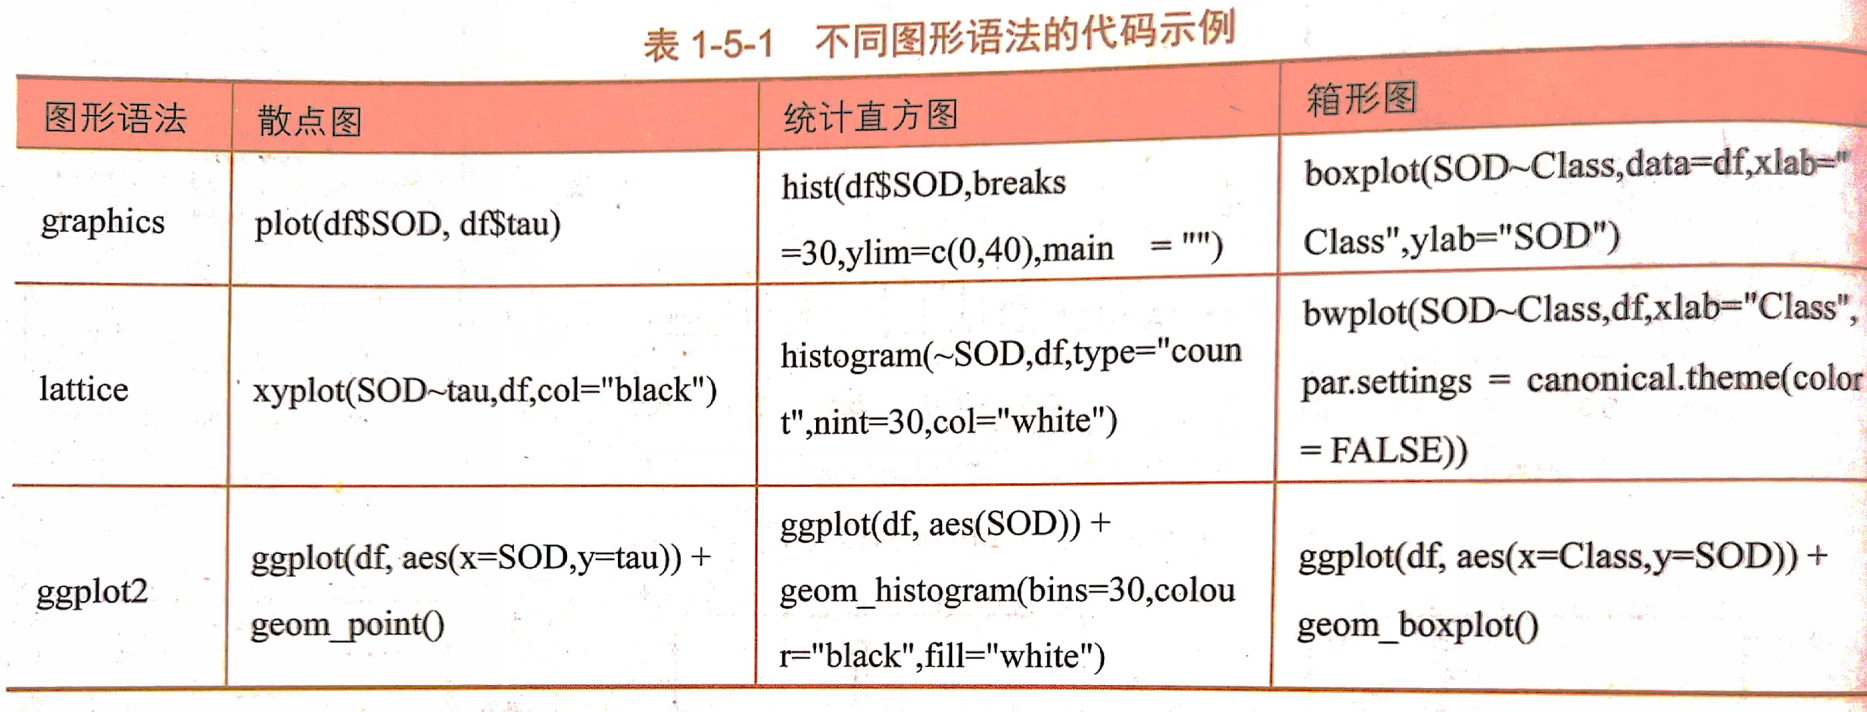
\includegraphics[width=0.8\textwidth]{screenshot004}
\end{figure}
\begin{lstlisting}[language=r]
> da <- read.csv("E:/11.R/R语言数据可视化之美/Beautiful-Visualization-with-R-master/第1章 R语言编程与绘图基础/Facet_Data.csv",stringsAsFactors=FALSE)
\end{lstlisting}

\subsection{lattice}

\begin{lstlisting}[language=r]
> library(lattice)
> p1<-xyplot(SOD~tau,da,col="black")
> 
> p2<-histogram(~SOD,da,type="count",nint=30,col="white")
> 
> 
> p3<-bwplot(SOD~Class,da,xlab="Class", 
+            par.settings = canonical.theme(color = FALSE))
> 
> library(gridExtra) 
> grid.arrange(p1,p2,p3, ncol = 3, nrow = 1)
\end{lstlisting}
\begin{figure}[H]
	\centering
	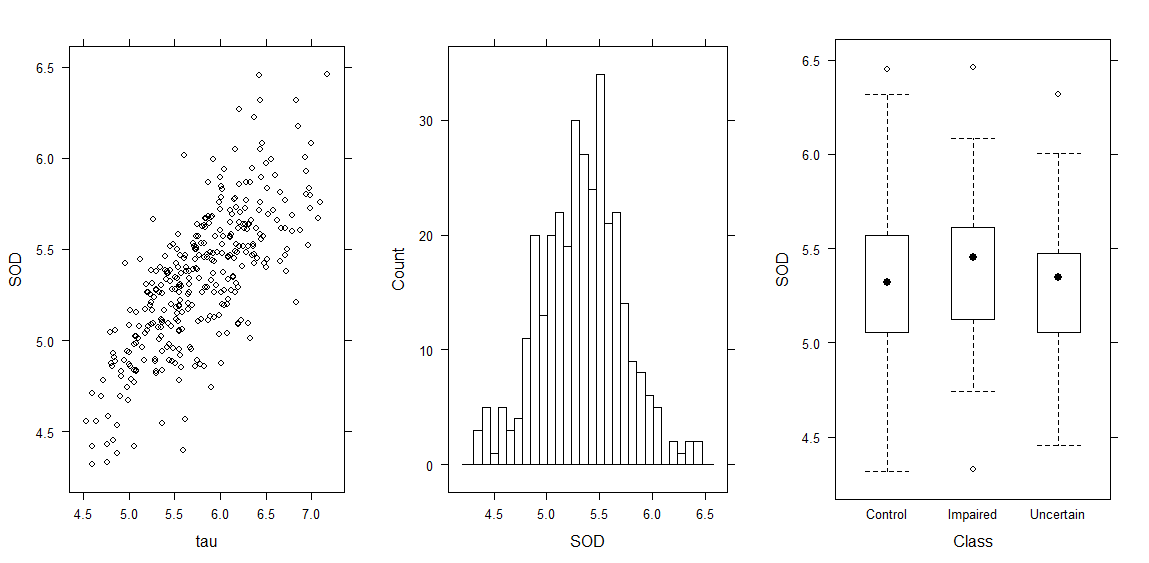
\includegraphics[width=\textwidth]{screenshot031}
\end{figure}


\subsection{base}
\begin{lstlisting}[language=r]
> par(mfrow=c(1,3))
> plot(da$SOD, da$tau)#,pch=21,lty=0.25,col="grey10") 
> hist(da$SOD,breaks =30,ylim=c(0,40),main  = "")
> boxplot(SOD~Class,data=da,xlab="Class",ylab="SOD")
\end{lstlisting}
\begin{figure}[H]
	\centering
	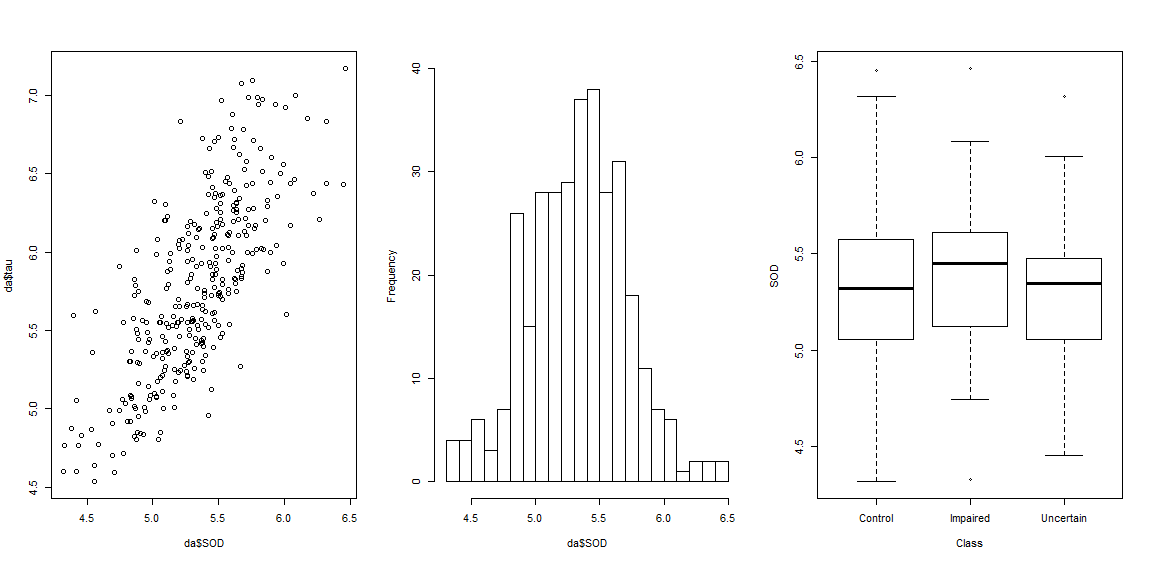
\includegraphics[width=\textwidth]{screenshot032}
\end{figure}
\subsection{ggplot2}

\begin{lstlisting}[language=r]
> library(ggplot2)
> 
> p1<-ggplot(da, aes(x=SOD,y=tau)) + 
+   geom_point() #shape=21,color="black",fill="red",size=3,stroke=0.1
> 
> p2<-ggplot(da, aes(SOD)) + 
+   geom_histogram(bins=30,colour="black",fill="white")
> 
> p3<-ggplot(da, aes(x=Class,y=SOD)) + 
+   geom_boxplot() 
> 
> library(gridExtra) 
> grid.arrange(p1,p2,p3, ncol = 3, nrow = 1)
\end{lstlisting}
\begin{figure}[H]
	\centering
	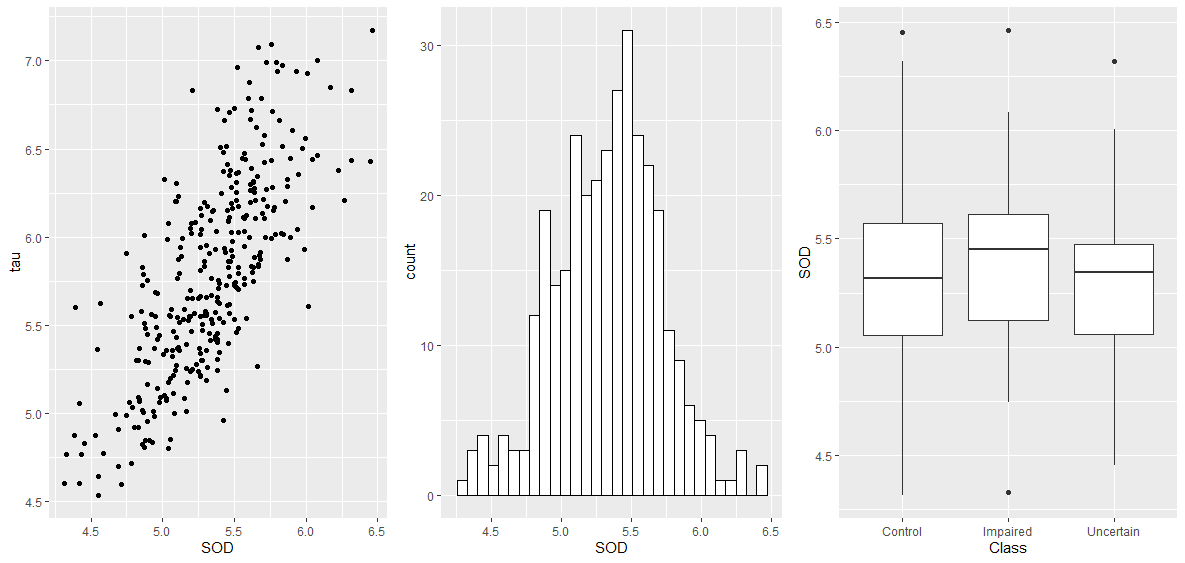
\includegraphics[width=\textwidth]{screenshot033}
\end{figure}

\section{ggplot2图形语法}

\begin{figure}[H]
	\centering
	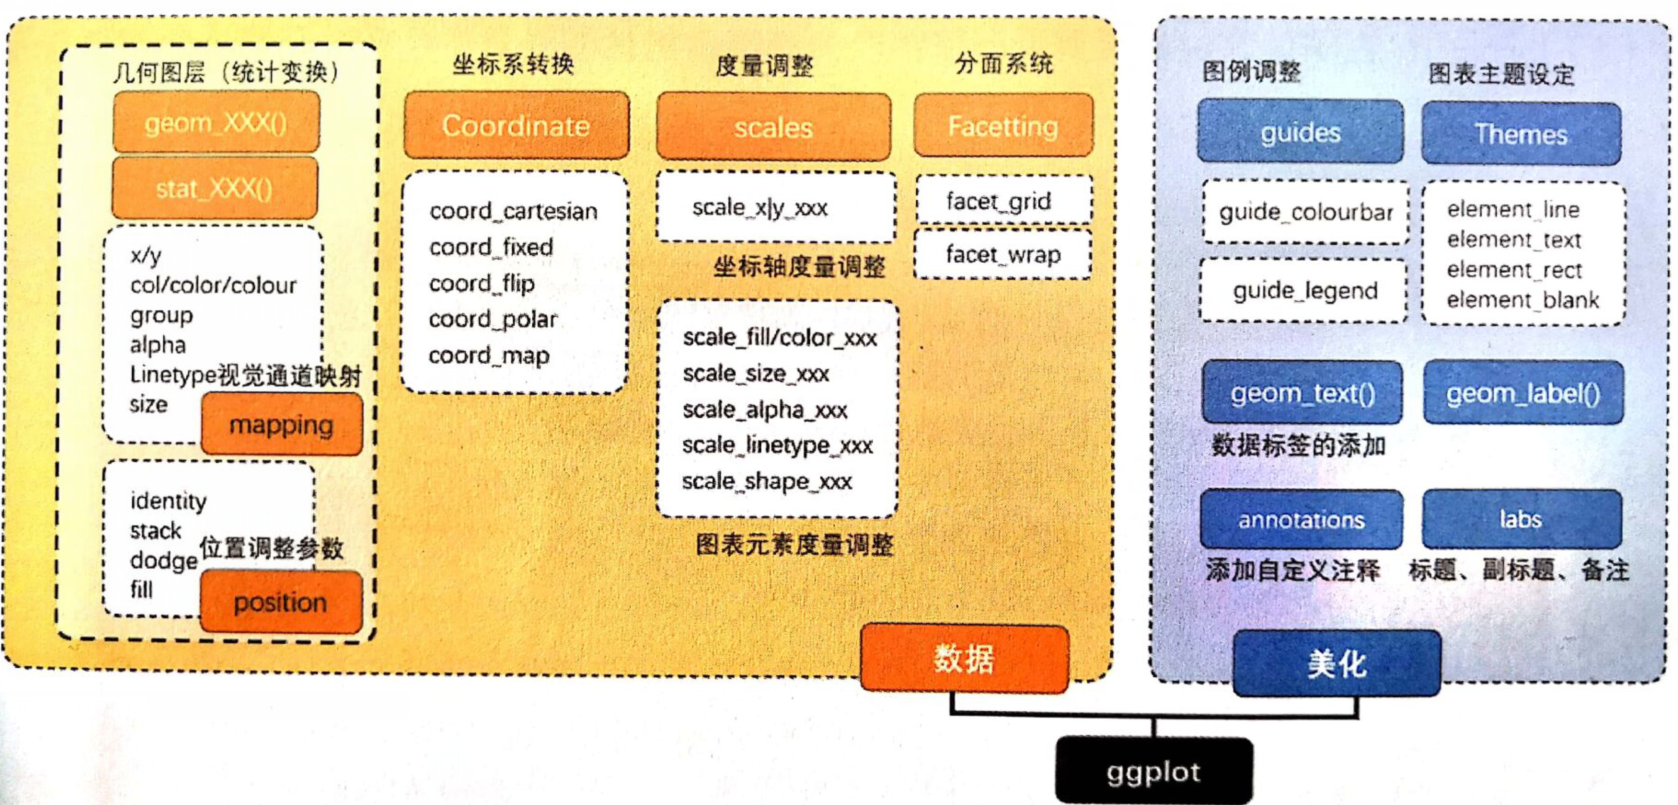
\includegraphics[width=0.9\textwidth]{screenshot005}
\end{figure}

\begin{figure}[H]
	\centering
	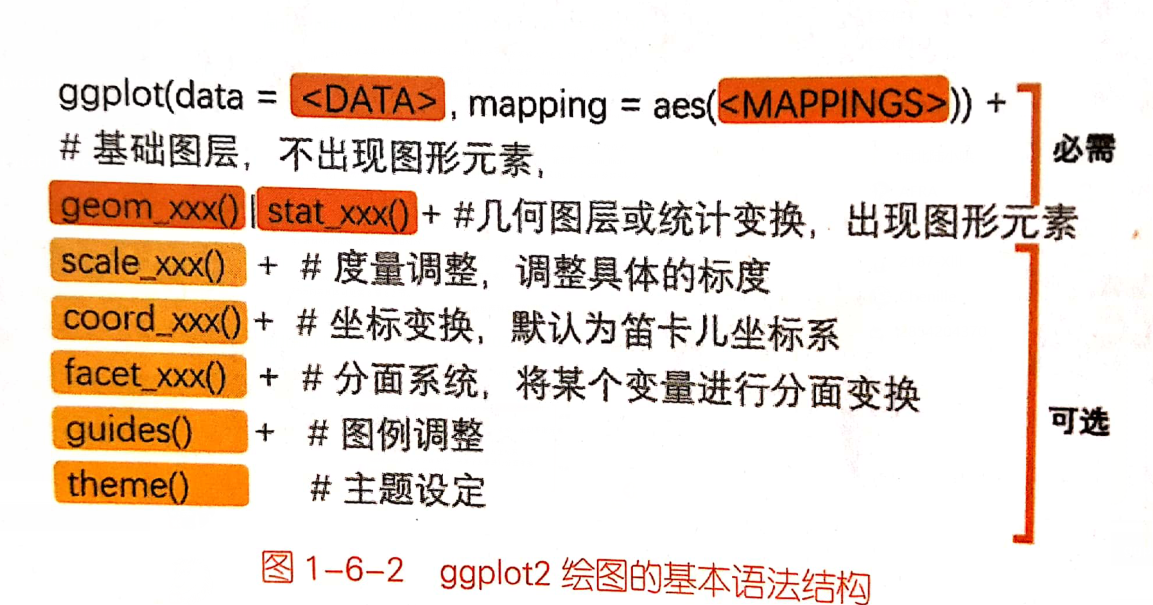
\includegraphics[width=0.6\textwidth]{screenshot016}
\end{figure}
%      

\subsection{视觉通道映射}
\begin{multicols}{2} 
\begin{lstlisting}[language=r]
> library(ggplot2)
> ggplot(da,aes(x=SOD,y=tau,size=age))+geom_point(shape=21,color="black",fill="#336A97",stroke=0.25)
\end{lstlisting}
\begin{figure}[H]
	\centering
	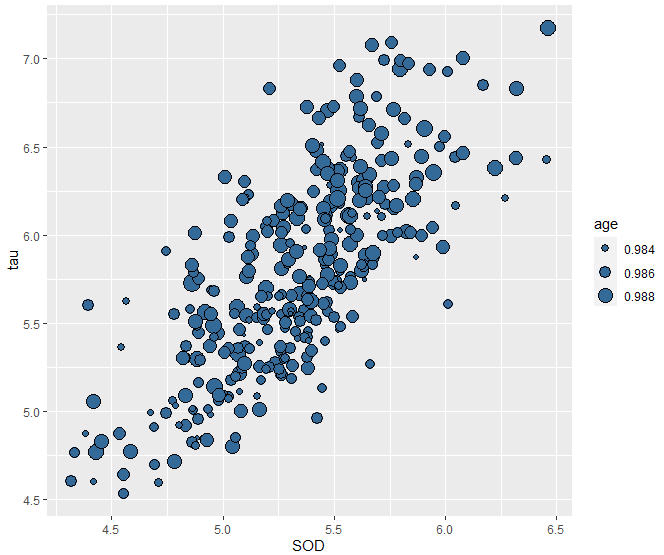
\includegraphics[width=0.5\textwidth]{screenshot018}
	\caption{age映射到散点的大小(size)}
	\label{fig:screenshot018}
\end{figure}
\end{multicols}
\begin{multicols}{2} 
\begin{lstlisting}[language=r]
> ggplot(da,aes(x=SOD,y=tau,fill=age,size=age))+geom_point(shape=21,color="black",stroke=0.25,alpha=0.8)
\end{lstlisting}
\begin{figure}[H]
	\centering
	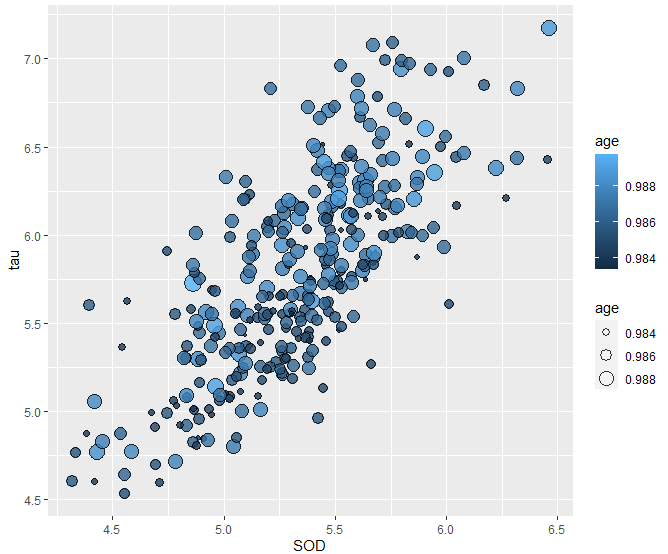
\includegraphics[width=0.5\textwidth]{screenshot017}
	\caption{age映射到散点的大小(size)和填充颜色(fill)}
	\label{fig:screenshot017}
\end{figure}
\end{multicols}
\begin{multicols}{2} 
\begin{lstlisting}[language=r]
> ggplot(da,aes(x=SOD,y=tau,fill=Class))+geom_point(shape=21,size=3,color="black",stroke=0.25)
\end{lstlisting}
\begin{figure}[H]
	\centering
	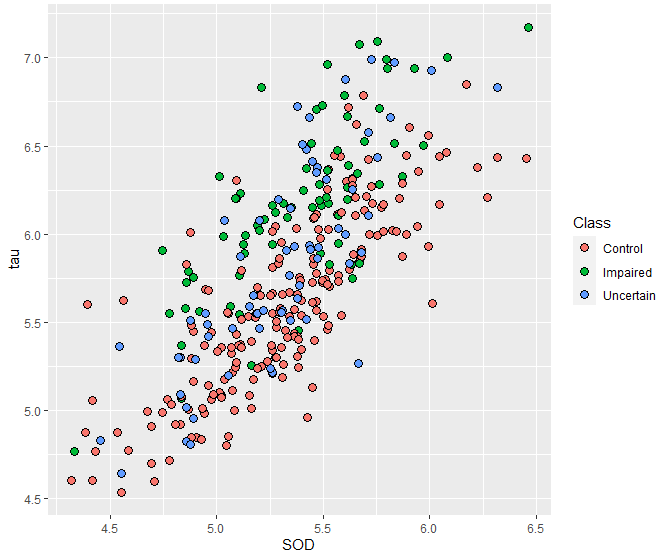
\includegraphics[width=0.5\textwidth]{screenshot019}
	\caption{Class映射到散点的填充颜色(fill)}
	\label{fig:screenshot019}
\end{figure}
\end{multicols}
\begin{multicols}{2} 
\begin{lstlisting}[language=r]
> ggplot(da,aes(x=SOD,y=tau,fill=Class,size=age))+geom_point(shape=21,color="black",stroke=0.25,alpha=0.8)
\end{lstlisting}
\begin{figure}[H]
	\centering
	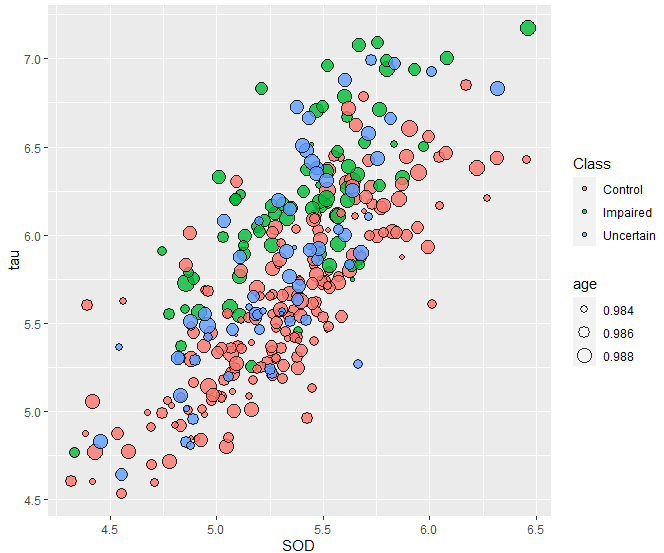
\includegraphics[width=0.5\textwidth]{screenshot020}
	\caption{age和Class分别映射到散点的大小和填充颜色}
	\label{fig:screenshot020}
\end{figure}
\end{multicols}

\subsubsection{比较重要的视觉通道映射}
字体(family),字型(fontface)
\begin{lstlisting}[language=r]
> x = seq(0,1,length.out = 4);y= seq(0,1,length.out = 3)
> x;y
[1] 0.0000000 0.3333333 0.6666667 1.0000000
[1] 0.0 0.5 1.0
> df <- expand.grid(x,y))
> df$fontface <-rep(c("plain", "bold", "italic", "bold.italic"),3)
> df$family<-rep(c("sans", "times",  "mono"),each=4)
> df$label<-paste(df$family,"\n ",df$fontface)

> ggplot(df, aes(x, y)) +
+   geom_text(aes(label = label, fontface = fontface,family=family),size = 4) +
+   xlim(-0.2,1.3)+
+   ylim(-0.2,1.2)
\end{lstlisting}
\begin{figure}[H]
	\centering
	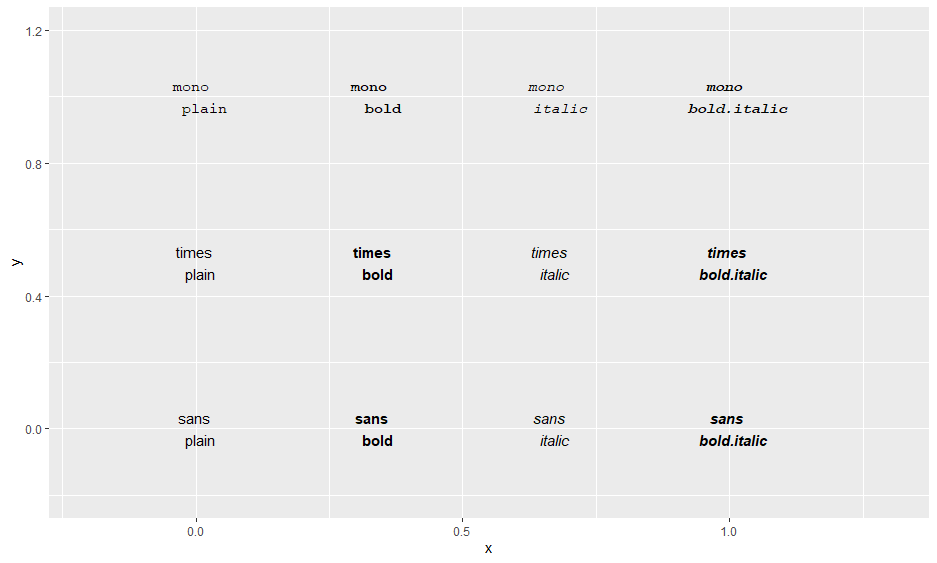
\includegraphics[width=\textwidth]{screenshot034}
\end{figure}

\subsection{度量控制}
\begin{multicols}{2}
\begin{lstlisting}[language=r]
> ggplot(da,aes(x=SOD,y=tau,size=age))+geom_point(shape=21,color="black",fill="#FF0000",stroke=0.25,alpha=0.8)+scale_size(range = c(1,8))
\end{lstlisting}
\begin{figure}[H]
	\centering
	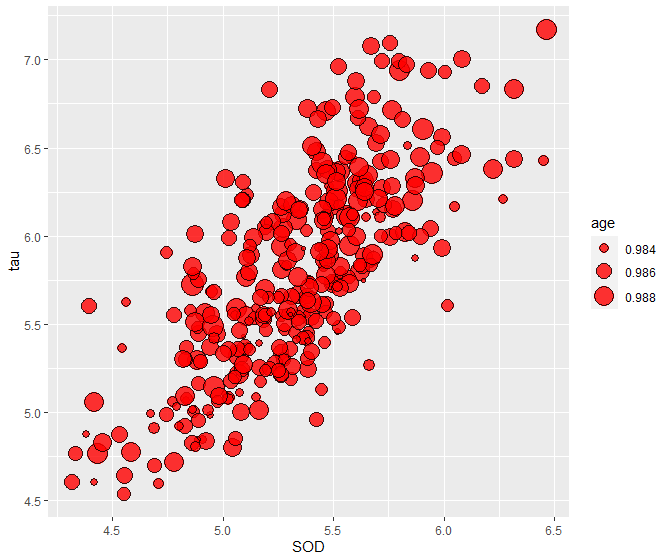
\includegraphics[width=0.5\textwidth]{screenshot021}
	\caption{散点大小的度量调整}
	\label{fig:screenshot021}
\end{figure}
\end{multicols}
\hspace{\fill}

\hspace{\fill}

\hspace{\fill}
\begin{multicols}{2}
\begin{lstlisting}[language=r]
> ggplot(da,aes(x=SOD,y=tau,size=age,fill=age))+geom_point(shape=21,color="black",stroke=0.25,alpha=0.8)+scale_size(range = c(1,8))+scale_fill_distiller(palette = "Reds",direction = 0)
\end{lstlisting}
\begin{figure}[H]
	\centering
	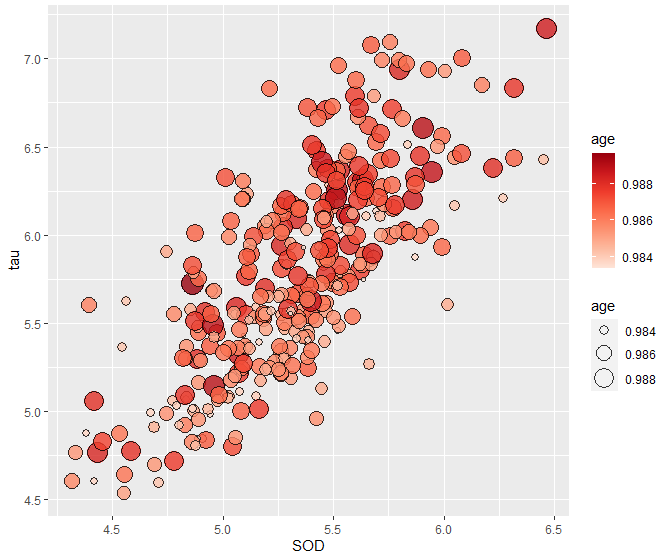
\includegraphics[width=0.5\textwidth]{screenshot022}
	\caption{散点大小和填充颜色的度量调整}
	\label{fig:screenshot022}
\end{figure}
\end{multicols}
\begin{multicols}{2}
\begin{lstlisting}[language=r]
> ggplot(da,aes(x=SOD,y=tau,fill=Class))+geom_point(shape=21,size=3,color="black",stroke=0.25)+scale_fill_manual(values = c("#36BED9","#FF0000","#FBAD01"))+scale_shape_manual(values = c(21,22,23))
\end{lstlisting}
\begin{figure}[H]
	\centering
	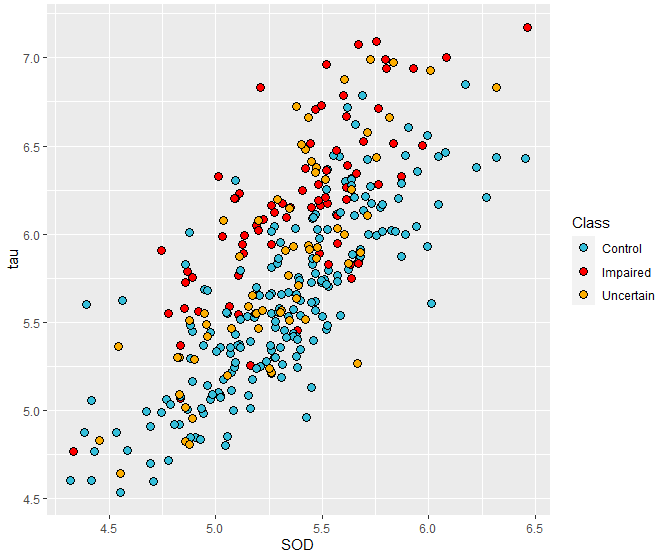
\includegraphics[width=0.5\textwidth]{screenshot023}
	\caption{散点填充颜色与形状的度量调整}
	\label{fig:screenshot023}
\end{figure}
\end{multicols}
\begin{multicols}{2}
\begin{lstlisting}[language=r]
> ggplot(da,aes(x=SOD,y=tau,fill=Class,size=age))+geom_point(shape=21,color="black",stroke=0.25,alpha=0.8)+scale_fill_manual(values = c("#36BED9","#FF0000","#FBAD01"))+scale_size(range=c(1,8))
\end{lstlisting}
\begin{figure}[H]
	\centering
	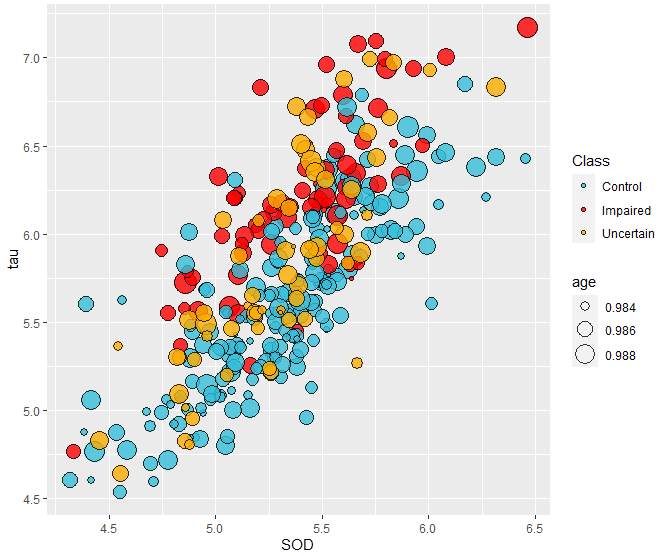
\includegraphics[width=0.5\textwidth]{screenshot024}
	\caption{散点大小和填充颜色的度量调整}
	\label{fig:screenshot024}
\end{figure}
\end{multicols}
\subsection{不同视觉暗示的组合结果}
\begin{multicols}{2}
\begin{lstlisting}[language=r]
> ggplot(data=da2,aes(x=Time,y=value,group=variable))+geom_line()+geom_point(shape=21,size=4,color="black",fill="white")+theme_classic()
\end{lstlisting}
\begin{figure}[H]
	\centering
	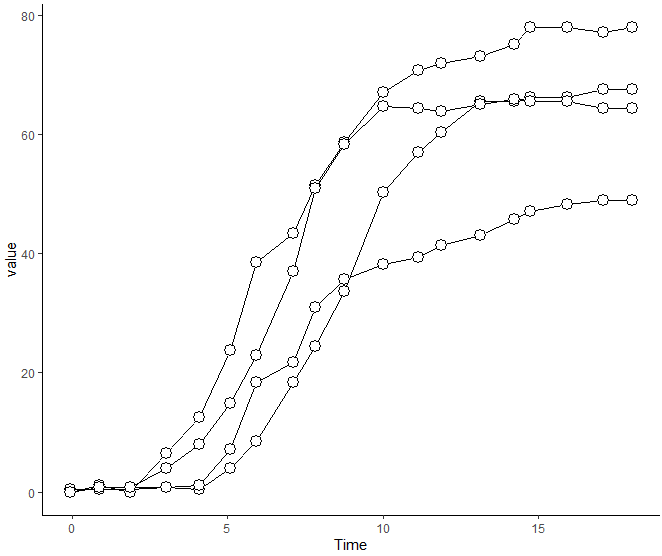
\includegraphics[width=0.5\textwidth]{screenshot025}
	\caption{位置+方向}
	\label{fig:screenshot025}
\end{figure}
\end{multicols}
\begin{multicols}{2}
\begin{lstlisting}[language=r]
> ggplot(data=da2,aes(x=Time,y=value,fill=variable))+geom_line()+geom_point(shape=21,size=4,color="black")+scale_fill_manual(values = c("grey60","grey30","black","white"))+theme_classic()
\end{lstlisting}
\begin{figure}[H]
	\centering
	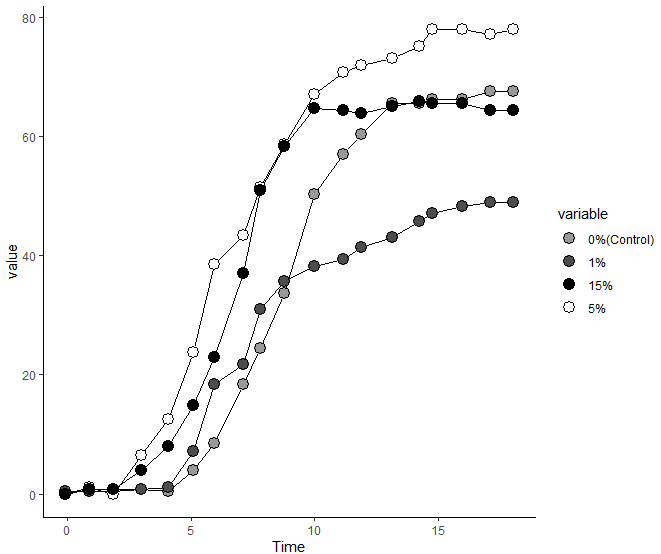
\includegraphics[width=0.5\textwidth]{screenshot026}
	\caption{位置+方向+饱和度}
	\label{fig:screenshot026}
\end{figure}
\end{multicols}
\begin{multicols}{2}
\begin{lstlisting}[language=r]
> ggplot(data=da2,aes(x=Time,y=value,shape=variable))+geom_line()+geom_point(size=4,color="black",fill="grey60")+scale_shape_manual(values = c(21,22,23,24))+theme_classic()
\end{lstlisting}
\begin{figure}[H]
	\centering
	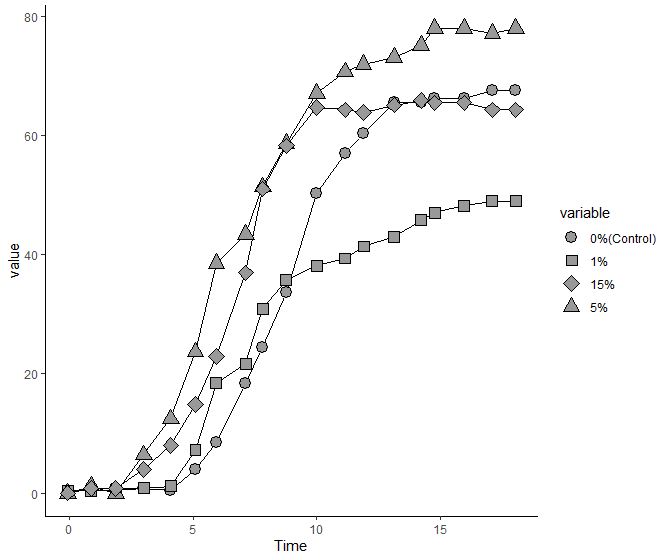
\includegraphics[width=0.5\textwidth]{screenshot027}
	\caption{位置+方向+形状}
	\label{fig:screenshot027}
\end{figure}
\end{multicols}
\begin{multicols}{2}
\begin{lstlisting}[language=r]
> ggplot(data=da2,aes(x=Time,y=value,fill=variable))+geom_line()+geom_point(shape=21,size=4,color="black")+scale_fill_manual(values = c("#FF9641","#FF5B4E","#B887C3","#38C25D"))+theme_classic()
\end{lstlisting}
\begin{figure}[H]
	\centering
	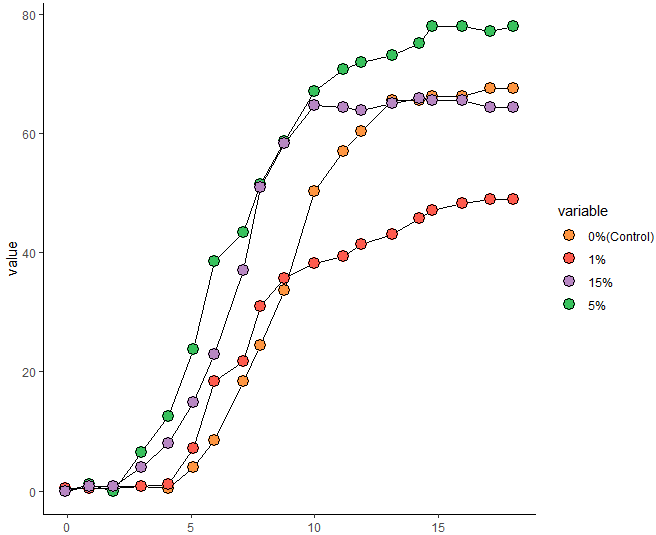
\includegraphics[width=0.5\textwidth]{screenshot028}
	\caption{位置+方向+色相}
	\label{fig:screenshot028}
\end{figure}
\end{multicols}
\begin{multicols}{2}
\begin{lstlisting}[language=r]
> ggplot(data=da2,aes(x=Time,y=value,fill=variable,shape=variable))+geom_line()+geom_point(size=4,color="black")+scale_fill_manual(values = c("grey60","grey30","black","white"))+scale_shape_manual(values = c(21,22,23,24))+theme_classic()
\end{lstlisting}
\begin{figure}[H]
	\centering
	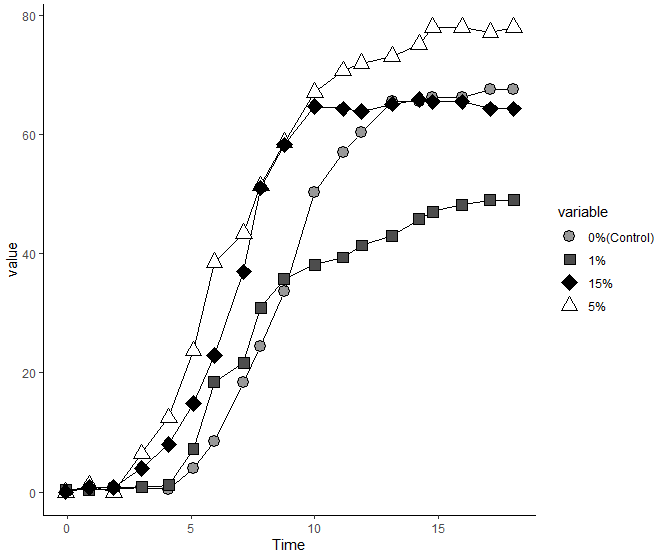
\includegraphics[width=0.5\textwidth]{screenshot029}
	\caption{位置+方向+饱和度+形状}
	\label{fig:screenshot029}
\end{figure}
\end{multicols}
\begin{multicols}{2}
\begin{lstlisting}[language=r]
> ggplot(data=da2,aes(x=Time,y=value,fill=variable,shape=variable))+geom_line()+geom_point(size=4,color="black")+scale_fill_manual(values = c("#FF9641","#FF5B4E","#B887C3","#38C25D"))+scale_shape_manual(values = c(21,22,23,24))+theme_classic()
\end{lstlisting}
\begin{figure}[H]
	\centering
	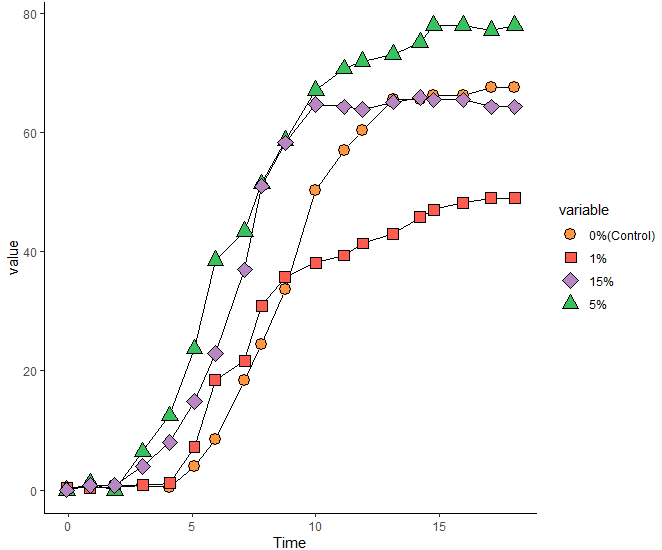
\includegraphics[width=0.5\textwidth]{screenshot030}
	\caption{位置+方向+色相+形状}
	\label{fig:screenshot030}
\end{figure}
\end{multicols}

\subsection{坐标系}
\subsubsection{三维直角坐标系的投影方法}
\begin{lstlisting}[language=r]
library(plot3D)
attach(quakes)
# Reference:https://github.com/coconn/cso002code_BrazilTradeOffsR

par(mfrow = c(1, 1))
panelfirst <- function(pmat) {
	zmin <- min(-quakes$depth)
	XY <- trans3D(quakes$long, quakes$lat,
	z = rep(zmin, nrow(quakes)), pmat = pmat)
	scatter2D(XY$x, XY$y, col = "black", pch = ".",
	cex = 2, add = TRUE, colkey = FALSE)
	xmin <- min(quakes$long)
	XY <- trans3D(x = rep(xmin, nrow(quakes)), y = quakes$lat,
	z = -quakes$depth, pmat = pmat)
	scatter2D(XY$x, XY$y, col = "black", pch = ".",
	cex = 2, add = TRUE, colkey = FALSE)
}

library(scales)
library(RColorBrewer)
library(fields) 
colormap <- colorRampPalette(rev(brewer.pal(11,'RdYlGn')))(100)#

index <- ceiling(((prc <- 0.7 * quakes$mag/ diff(range(quakes$mag))) - min(prc) + 0.3)*100)
for (i in seq(1,length(index)) ){
	prc[i]=colormap[index[i]]
}

pmar <- par(mar = c(5.1, 4.1, 4.1, 6.1))
with(quakes, scatter3D(x = long, y = lat, z = -depth, bgvar = mag,
pch = 21, cex = 1.5,col="black",bg=prc,
xlab = "longitude", ylab = "latitude",
zlab = "depth, km", 
ticktype = "detailed",bty = "f",box = TRUE,
panel.first = panelfirst,
theta = 140, phi = 20, d=1.5,
colkey = FALSE,
list(length = 0.5, width = 0.5, cex.clab = 0.75))

colkey (col=colormap,clim=range(quakes$mag),clab = "Richter", add=TRUE, length=0.5,side = 4)

#--------------------------------------------------------------------
pmar <- par(mar = c(5.1, 4.1, 4.1, 6.1))
with(quakes, scatter3D(x = long, y = lat, z = -depth, #bgvar = mag,
pch = 21, cex = 1.5,col="black",bg=prc,
xlab = "longitude", ylab = "latitude",
zlab = "depth, km", 
ticktype = "detailed",bty = "f",box = TRUE,
panel.first = panelfirst,
theta = 140, phi = 20, d=3,
colkey = FALSE)#list(length = 0.5, width = 0.5, cex.clab = 0.75))
)
colkey (col=colormap,clim=range(quakes$mag),clab = "Richter", add=TRUE, length=0.5,side = 4)

#--------------------------------------------------------------------
pmar <- par(mar = c(5.1, 4.1, 4.1, 6.1))
with(quakes, scatter3D(x = long, y = lat, z = -depth, #bgvar = mag,
pch = 21, cex = 1.5,col="black",bg=prc,
xlab = "longitude", ylab = "latitude",
zlab = "depth, km", 
ticktype = "detailed",#bty = "f",box = TRUE,
panel.first = panelfirst,
theta = 140, phi = 20, d=30,
colkey = FALSE)#list(length = 0.5, width = 0.5, cex.clab = 0.75))
)
colkey (col=colormap,clim=range(quakes$mag),clab = "Richter", add=TRUE, length=0.5,side = 4)
\end{lstlisting}
\begin{figure}[H]
	\centering
	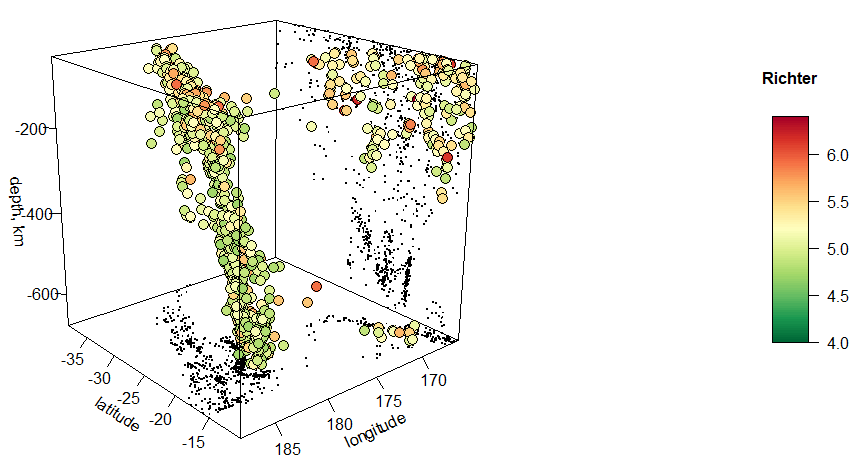
\includegraphics[width=\textwidth]{screenshot035}
	\caption{透视投影}
	\label{fig:screenshot035}
\end{figure}
\begin{figure}[H]
	\centering
	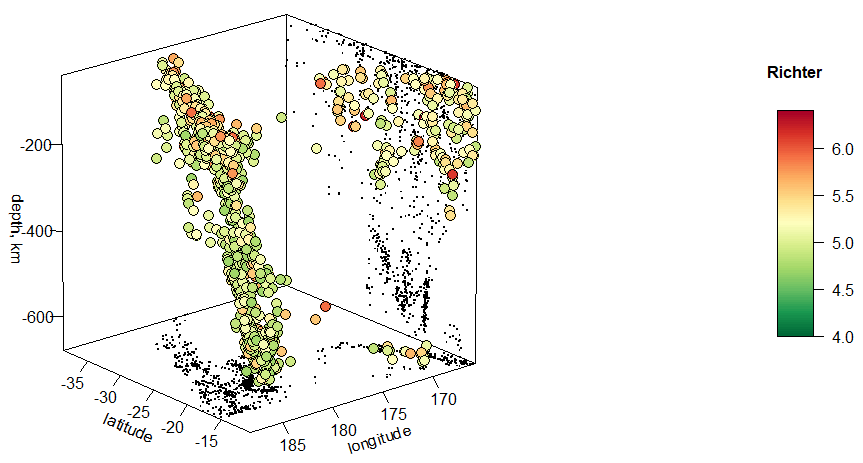
\includegraphics[width=\textwidth]{screenshot036}
	\caption{正交投影}
	\label{fig:screenshot036}
\end{figure}

\subsubsection{坐标系的转换}
\begin{lstlisting}[language=r]
> setwd("E:/11.R/R语言数据可视化之美/Beautiful-Visualization-with-R-master/第1章 R语言编程与绘图基础")
> library(ggplot2)
> df<-read.csv("PolarBar_Data.csv", header = TRUE)
> ggplot(df,aes(Date,Value))+
+   geom_bar(stat = "identity", width = 10,colour="black",size=0.25,fill="#3BC8EB")+ #离散柱形图
+   scale_x_continuous(name="Time(day)",breaks=seq(0,360,30))+
+   scale_y_continuous(breaks=seq(0,160,20),limits=c(0,160),expand = expand_scale(add = 0))+
+   theme_classic()
\end{lstlisting}
\begin{figure}[H]
	\centering
	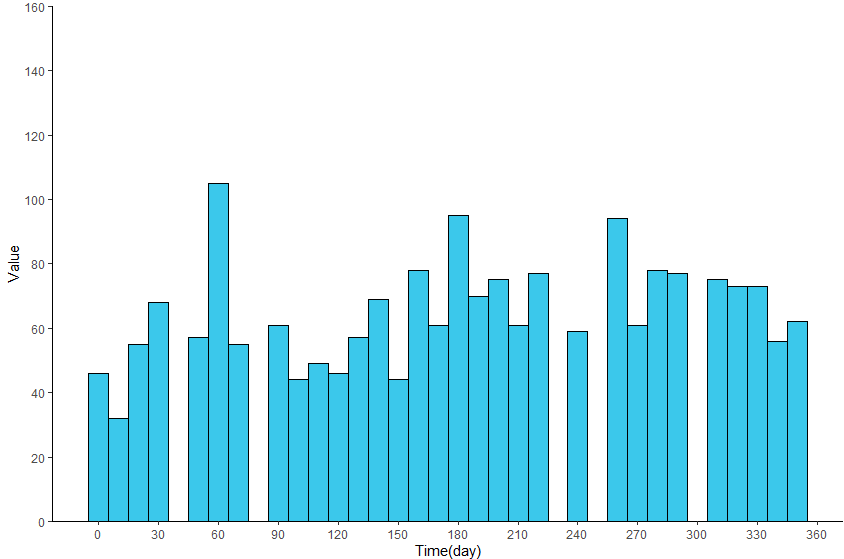
\includegraphics[width=0.5\textwidth]{screenshot037}
	\caption{直角坐标系柱形图}
	\label{fig:screenshot037}
\end{figure}

\begin{lstlisting}[language=r]
> ggplot(df,aes(Date,Value))+
+   geom_bar(stat = "identity", width = 10,colour="black",size=0.25,fill="#3BC8EB")+
+   scale_x_continuous(breaks=seq(0,360,30))+
+   scale_y_continuous(breaks=seq(0,115,30),limits=c(-30,115))+
+   coord_polar(theta = "x",start=0) +
+   theme_light()+
+   theme( panel.background = element_blank(),
+          panel.grid.major = element_line(colour = "grey80",size=.25),
+          axis.text.y = element_text(size = 11,colour="black"),
+          axis.line.y = element_line(size=0.25),
+          axis.text.x=element_text(size = 11,colour="black"))
\end{lstlisting}
\begin{figure}[H]
	\centering
	
\includegraphics[width=0.5\textwidth]{screenshot001}
	\caption{极坐标系柱形图}
	\label{fig:screenshot001}
\end{figure}

\begin{lstlisting}[language=r]
> df2<-read.csv("PolarArea_Data.csv", header = TRUE)
> 
> ggplot(df2,aes(Date,Value))+
+   geom_area(colour="black",size=0.25,fill="#FFA1B9")+
+   scale_x_continuous(name="Time(day)",breaks=seq(0,360,60),expand = expand_scale(add = 0))+
+   scale_y_continuous(breaks=seq(0,3500,500),limits=c(0,3500),expand = expand_scale(add = 0))+
+   theme_classic()
\end{lstlisting}
\begin{figure}[H]
	\centering
	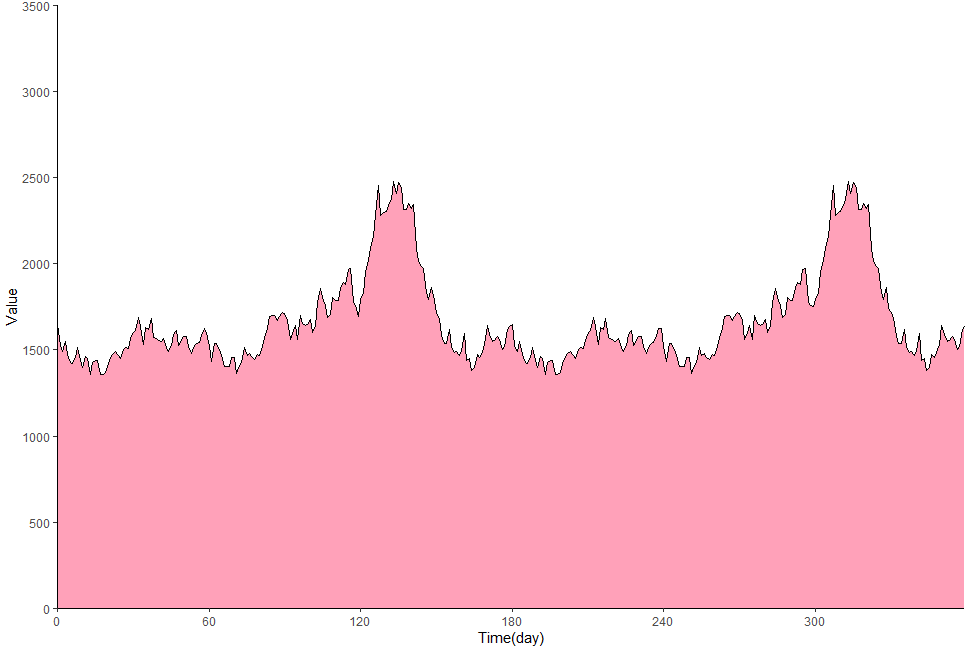
\includegraphics[width=0.5\textwidth]{screenshot002}
	\caption{直角坐标系面积图}
	\label{fig:screenshot002}
\end{figure}

\begin{lstlisting}[language=r]
> ggplot(df2,aes(Date,Value))+
+   geom_area(colour=NA,size=0.25,fill="#FFA1B9",alpha=0.7)+
+   geom_line(colour="black",size=0.25)+
+   scale_x_continuous(name="Time(day)",breaks=seq(0,360,30))+
+   scale_y_continuous(breaks=seq(0,3000,500),limits=c(0,3000))+
+   coord_polar(theta = "x",start=0) +
+   theme_light()+
+   theme( panel.background = element_blank(),
+          panel.grid.major = element_line(colour = "grey80",size=.25),
+          axis.text.y = element_text(size = 10,colour="black"),
+          axis.line.y = element_line(size=0.25),
+          axis.text.x=element_text(size = 11,colour="black"))
\end{lstlisting}
\begin{figure}[H]
	\centering
	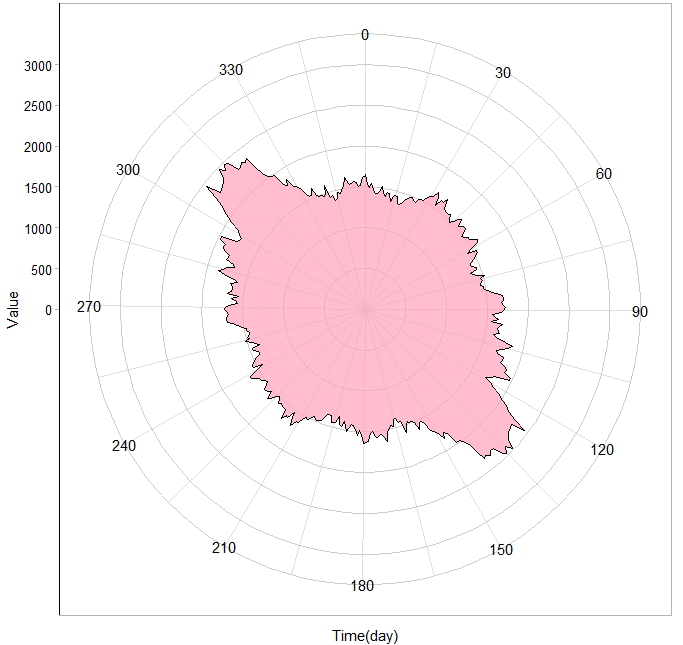
\includegraphics[width=0.5\textwidth]{screenshot003}
	\caption{极坐标系面积图}
	\label{fig:screenshot003}
\end{figure}

\subsubsection{直角坐标系度量的调整}
\begin{lstlisting}[language=r]
> library(ggplot2)
> library(RColorBrewer)
> library(reshape2)
> df<-read.csv("MappingAnalysis_Data.csv", header = TRUE)
> ggplot(data=df, aes(x=Time,y=value,fill=variable,shape=variable)) + 
+   geom_line()+
+   geom_point(size=4,colour="black") +
+   scale_fill_manual(values=c("#FF9641","#FF5B4E","#B887C3","#38C25D"))+
+   scale_shape_manual(values=c(21,22,23,24))+
+   theme_classic()+
+   theme(
+     text=element_text(size=14,color="black"),
+     plot.title=element_text(size=14,family="myfont",face="bold.italic",hjust=.5,color="black"),
+     legend.background = element_blank(),
+     legend.position=c(0.2,0.8)
+   )
\end{lstlisting}
\begin{figure}[H]
	\centering
	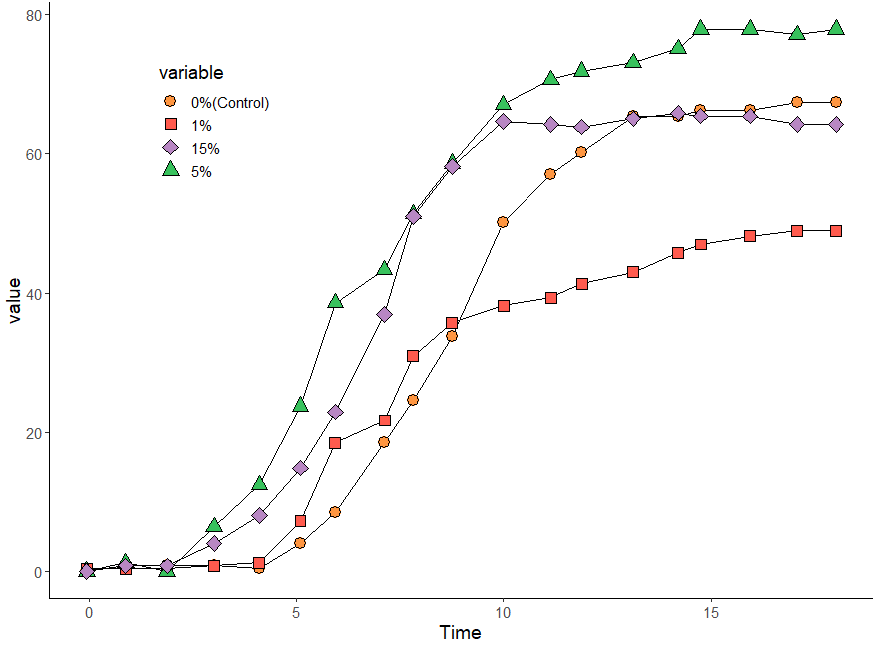
\includegraphics[width=0.5\textwidth]{screenshot006}
\end{figure}

\begin{lstlisting}[language=r]
> ggplot(data=df, aes(x=Time,y=value,fill=variable,shape=variable)) + 
+   geom_line()+
+   geom_point(size=4,colour="black") +
+   scale_fill_manual(values=c("#FF9641","#FF5B4E","#B887C3","#38C25D"))+
+   scale_shape_manual(values=c(21,22,23,24))+
+   
+   scale_x_continuous(name="Time(d)",breaks=seq(0,20,2))+
+   scale_y_continuous(breaks=seq(0,90,10),limits=c(0,90),expand =c(0, 1))+
+   
+   theme_classic()+
+   theme(
+     text=element_text(size=14,color="black"),
+     plot.title=element_text(size=14,family="myfont",face="bold.italic",hjust=.5,color="black"),
+     legend.background = element_blank(),
+     legend.position=c(0.2,0.8)
+   )
\end{lstlisting}
\begin{figure}[H]
	\centering
	
\includegraphics[width=0.5\textwidth]{screenshot007}
\end{figure}

\subsection{图例}
\begin{lstlisting}[language=r]
> ggplot(data=df, aes(x=Time,y=value,fill=variable,shape=variable)) + 
+   geom_line()+
+   geom_point(size=4,colour="black") +
+   scale_fill_manual(values=c("#FF9641","#FF5B4E","#B887C3","#38C25D"))+
+   scale_shape_manual(values=c(21,22,23,24))+
+   
+   scale_x_continuous(name="Time(d)",breaks=seq(0,20,2))+
+   scale_y_continuous(breaks=seq(0,90,10),limits=c(0,90),expand =c(0, 1))+
+   
+   theme_classic()+
+   theme(
+     text=element_text(size=14,color="black"),
+     legend.background = element_rect(fill="white"),
+     legend.position="right"
+   )
\end{lstlisting}
\begin{figure}[H]
	\centering
	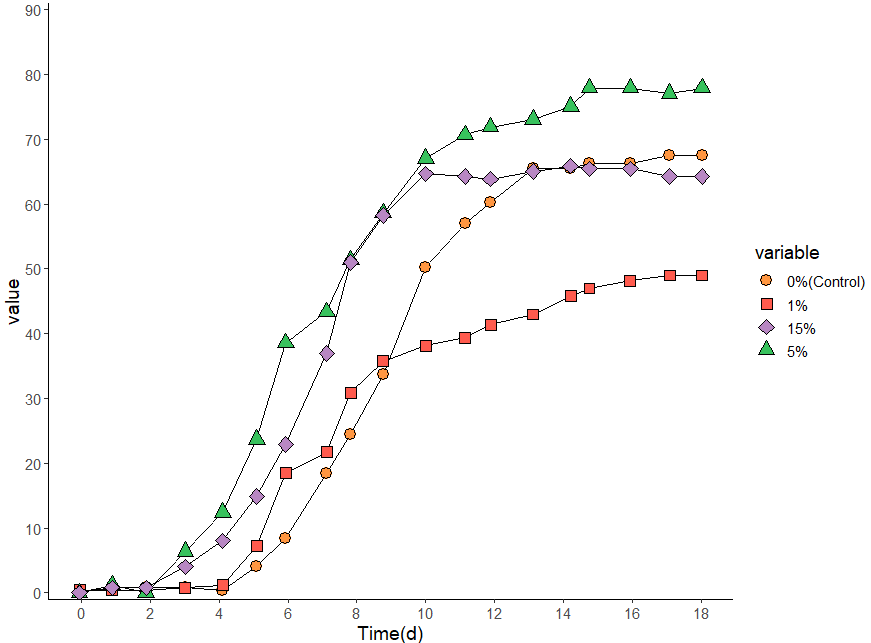
\includegraphics[width=0.5\textwidth]{screenshot008}
\end{figure}

\begin{lstlisting}[language=r]
> ggplot(data=df, aes(x=Time,y=value,fill=variable,shape=variable)) + 
+   geom_line()+
+   geom_point(size=4,colour="black") +
+   scale_fill_manual(values=c("#FF9641","#FF5B4E","#B887C3","#38C25D"))+
+   scale_shape_manual(values=c(21,22,23,24))+
+   
+   scale_x_continuous(name="Time(d)",breaks=seq(0,20,2))+
+   scale_y_continuous(breaks=seq(0,90,10),limits=c(0,90),expand =c(0, 1))+
+   
+   theme_classic()+
+   theme(
+     text=element_text(size=14,color="black"),
+    legend.background = element_blank(),
+     legend.position=c(0.2,0.8)
+   )
\end{lstlisting}
\begin{figure}[H]
	\centering
	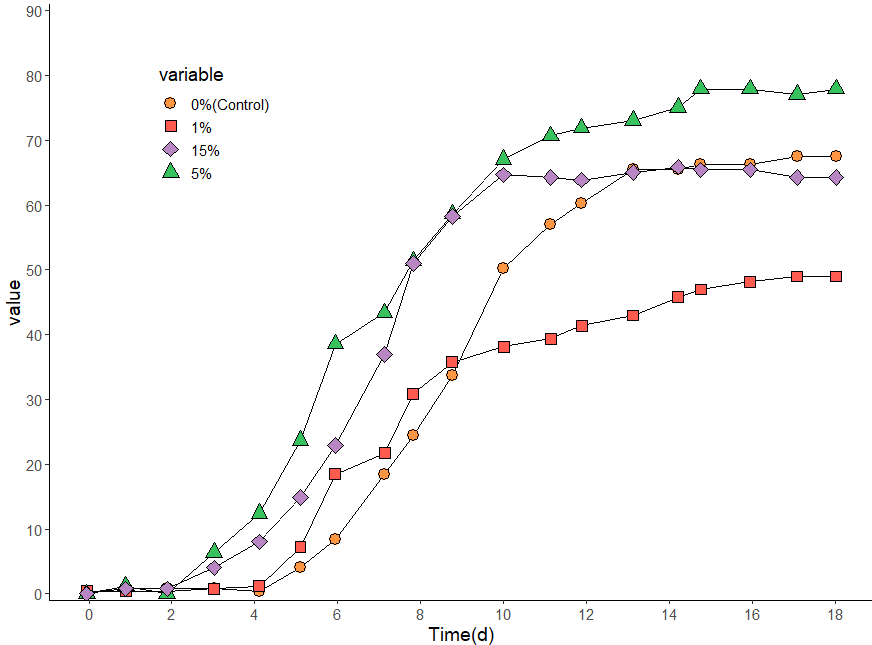
\includegraphics[width=0.5\textwidth]{screenshot009}
\end{figure}
\subsection{主题系统}
\subsubsection{ggThemeAssist包}
\begin{figure}[H]
	\centering
	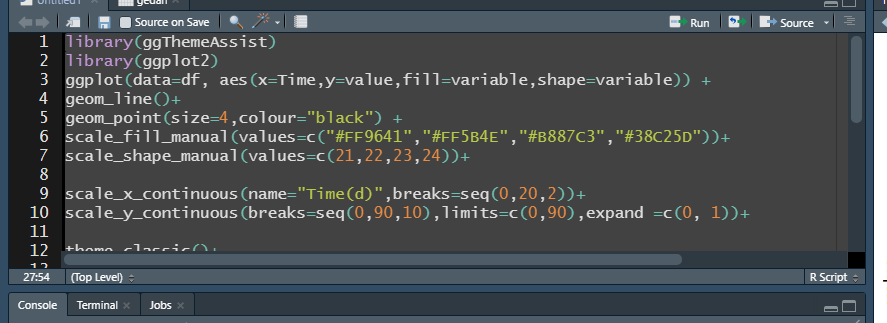
\includegraphics[width=0.8\textwidth]{screenshot012}
	\caption{选定你画好的ggplot}
	\label{fig:screenshot012}
\end{figure}

\begin{figure}[H]
	\centering
	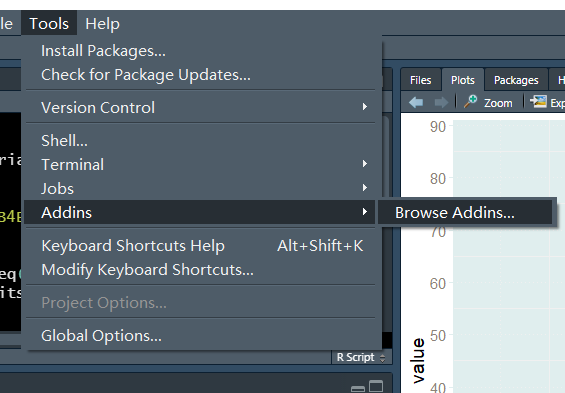
\includegraphics[width=0.5\textwidth]{screenshot010}
\end{figure}
\begin{figure}[H]
	\centering
	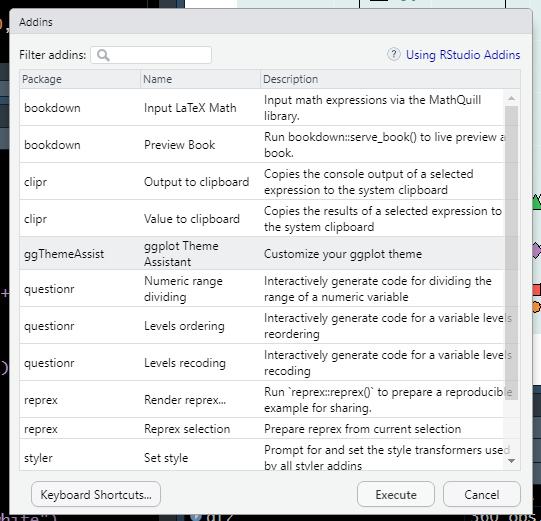
\includegraphics[width=0.5\textwidth]{screenshot011}
\end{figure}
\begin{figure}[H]
	\centering
	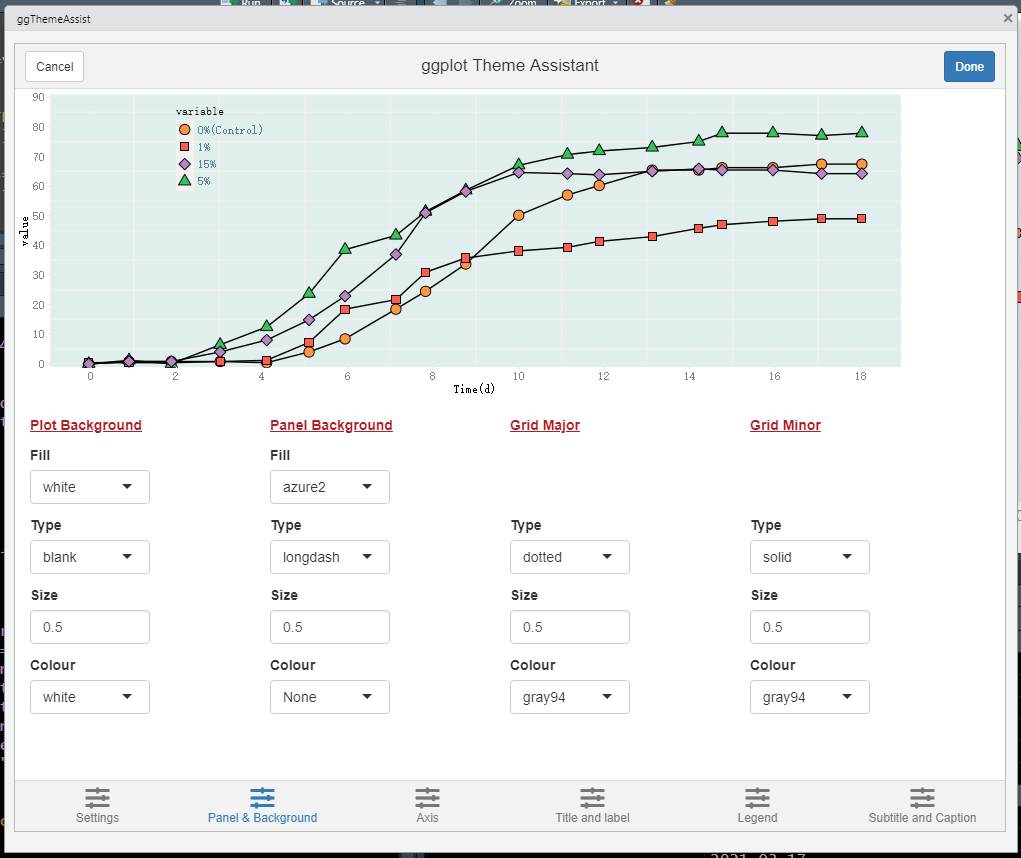
\includegraphics[width=0.5\textwidth]{screenshot013}
\end{figure}

\subsubsection{套用主题模板}

\begin{lstlisting}[language=r]
> library(ggplot2)
> library(wesanderson)
> 
> ggplot(iris,aes(Sepal.Length, Petal.Length, fill= Species))+
+   geom_point(size=3.5,shape=21,colour="black") +
+   scale_fill_manual(values=wes_palette(n=3, name="Darjeeling1"))+
+   theme_light()

> #----------------------------Python---------------------------
> ggplot(iris,aes(Sepal.Length, Petal.Length, fill= Species))+
+   geom_point(size=3.5,shape=21,colour="black") +
+   scale_fill_manual(values=wes_palette(n=3, name="Darjeeling1"))+
+   theme_minimal()
\end{lstlisting}
\begin{figure}[H]
	\centering
	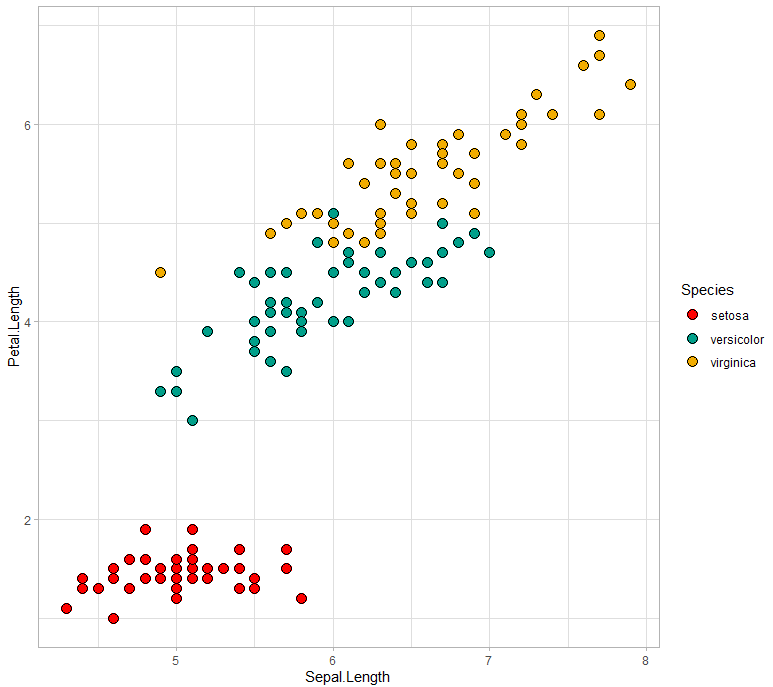
\includegraphics[width=0.5\textwidth]{screenshot014}
	\caption{theme$ \_ $light()}
	\label{fig:screenshot014}
\end{figure}
\begin{figure}[H]
	\centering
	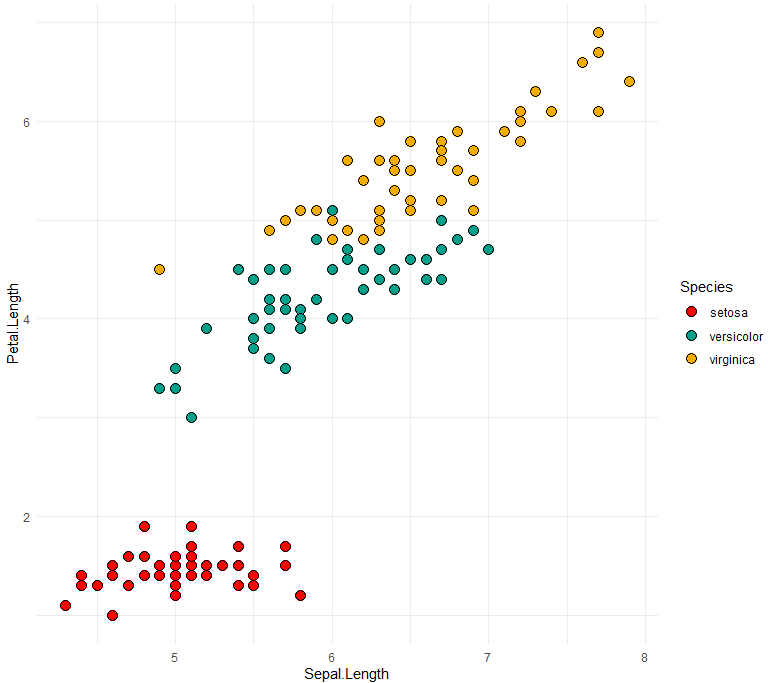
\includegraphics[width=0.5\textwidth]{screenshot038}
	\caption{theme$ \_ $minimal()}
	\label{fig:screenshot038}
\end{figure}
\subsection{位置调整}
\begin{lstlisting}[language=r]
> N <- 100
> df <- data.frame(group=rep(c(1,2),each=N*2),
+ y=append(append(rnorm(N,5,1),rnorm(N,2,1)),append(rnorm(N,1,1),rnorm(N,3,1))),
+                  x=rep(c("A","B","A","B"),N))
\end{lstlisting}
\begin{lstlisting}[language=r]
> ggplot(df,aes(x=x,y=y,fill=as.factor(group)))+
+   geom_boxplot(outlier.size = 0,color="black")+
+   geom_jitter(aes(group=as.factor(group)),shape=21,alpha=0.5)
\end{lstlisting}
\begin{figure}[H]
	\centering
	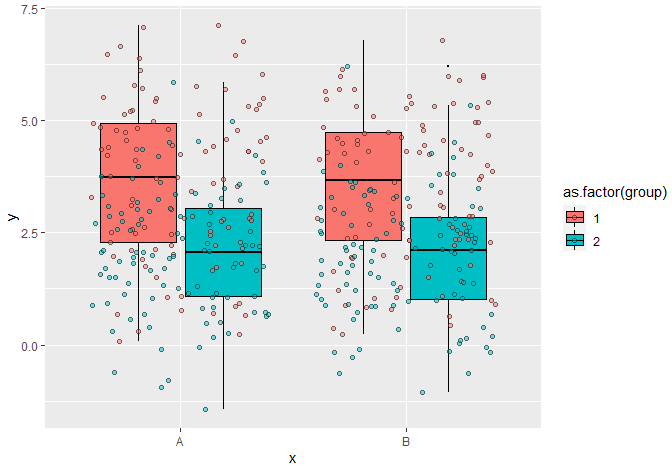
\includegraphics[width=0.5\textwidth]{screenshot039}
\end{figure}

\begin{lstlisting}[language=r]
> ggplot(df,aes(x=x,y=y,fill=as.factor(group)))+
+   geom_boxplot(outlier.size = 0,color="black")+
+   geom_jitter(aes(group=as.factor(group)),shape=21,alpha=0.5,position = position_jitterdodge())
\end{lstlisting}
\begin{figure}[H]
	\centering
	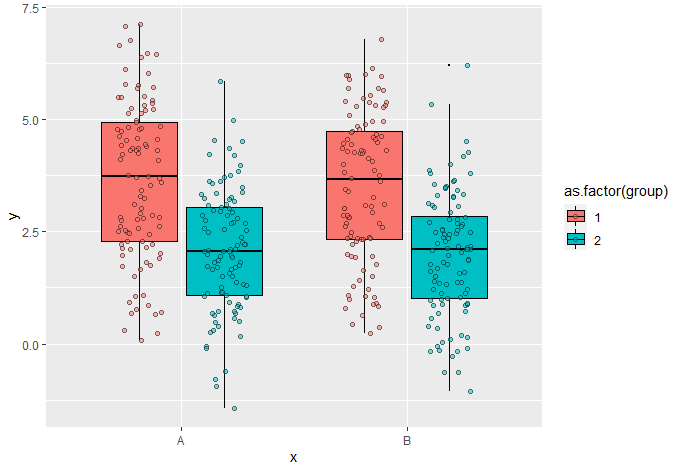
\includegraphics[width=0.5\textwidth]{screenshot040}
\end{figure}

\begin{lstlisting}[language=r]
> ggplot(df,aes(x=x,y=y,fill=as.factor(group)))+
+   geom_boxplot(position=position_dodge(0.75),outlier.size = 0,color="black")+
+   geom_jitter(aes(group=as.factor(group)),shape=21,alpha=0.5,position = position_jitterdodge(dodge.width = 0.75))
\end{lstlisting}
\begin{figure}[H]
	\centering
	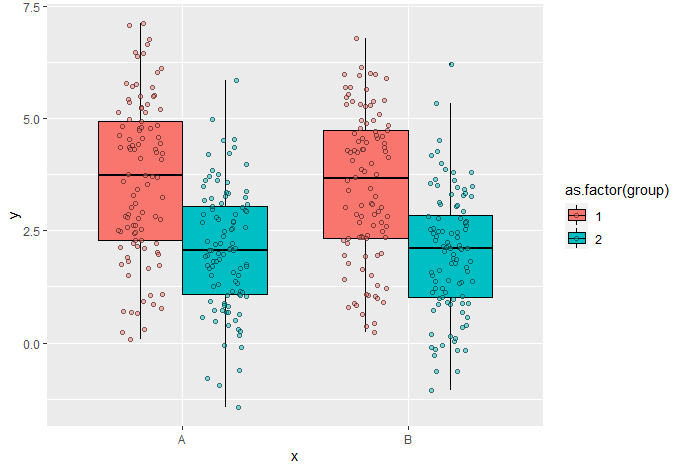
\includegraphics[width=0.5\textwidth]{screenshot041}
\end{figure}
\subsection{交互操作实现简单的ggplot}
\begin{figure}[H]
	\centering
	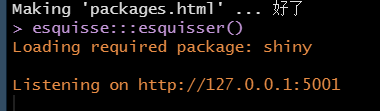
\includegraphics[width=0.5\textwidth]{screenshot042}
\end{figure}
\begin{figure}[H]
	\centering
	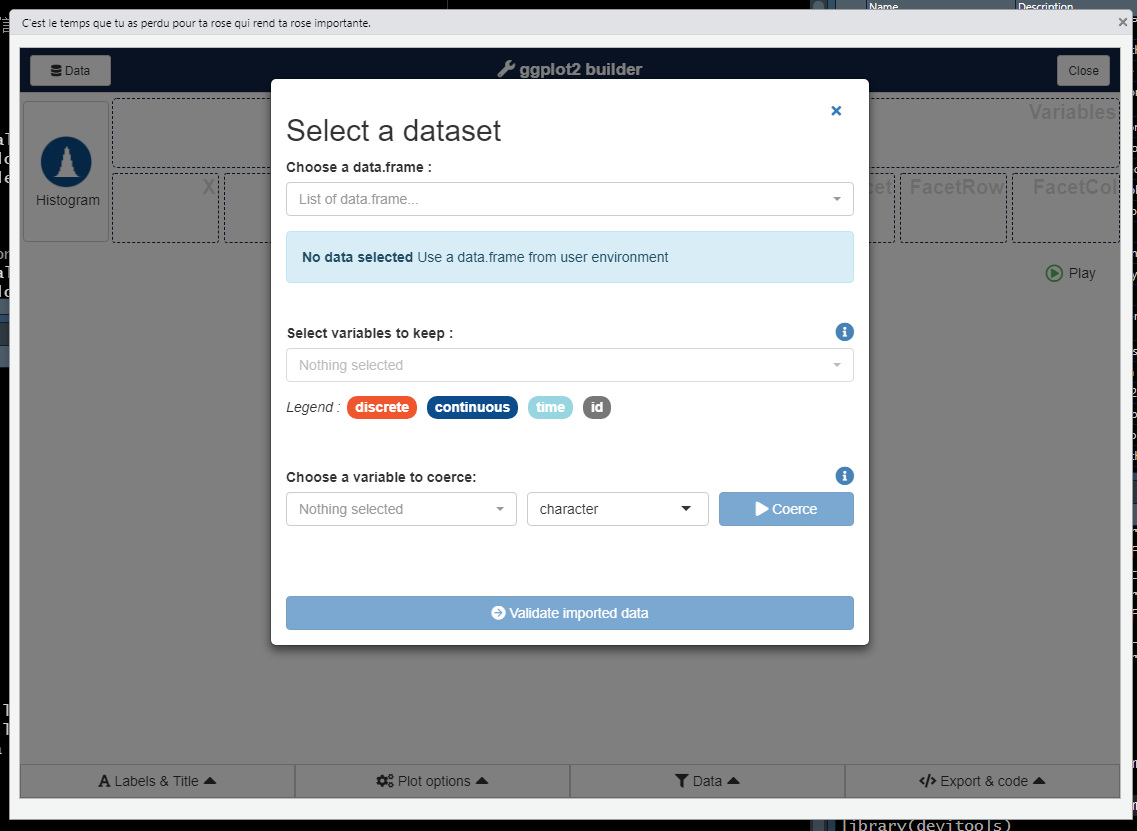
\includegraphics[width=0.8\textwidth]{screenshot043}
\end{figure}
\subsection{高手必备}
特别强调的是,要想熟练使用ggplot2,就必须深入理解ggplot与geom对象之间的关系. P61
\begin{lstlisting}[language=r]
library(ggplot2)
N <- 20
df1 <- data.frame(x=sort(rnorm(N)),y=sort(rnorm(N)))
df2 <- data.frame(x=df1$x+0.1*rnorm(N),y=df1$y+0.1*rnorm(N))

p1 <- ggplot(df1,aes(x,y,color=x+y))+
geom_line(size=1)+
geom_point(shape=16,size=5)+
guides(color=guide_colorbar(title = "Point\nLine"))+
labs(title = "所有图层共享数据源和视觉通道映射")

p2 <- ggplot(df1,aes(x,y))+
geom_line(aes(color=x+y),size=1)+
geom_point(aes(fill=x+y),size=5,color="black",shape=21)+
scale_fill_distiller(name="Point",palette="YlOrRd")+
scale_color_distiller(name="Line",palette = "Blues")+
labs(title="所有图层仅共享数据源")

p3 <- ggplot()+
geom_line(aes(x,y,color=x+y),df1,size=1)+
geom_point(aes(x,y,fill=x+y),df2,color="black",shape=21,size=5)+
scale_fill_distiller(name="Point",palette = "YlOrRd")+
scale_color_distiller(name="Line",palette = "Blues")+
labs(title="各图层对象均使用独立的数据源与视觉通道映射")

library(gridExtra) 
grid.arrange(p1,p2,p3, ncol = 3, nrow = 1)
\end{lstlisting}
\begin{figure}[H]
	\centering
	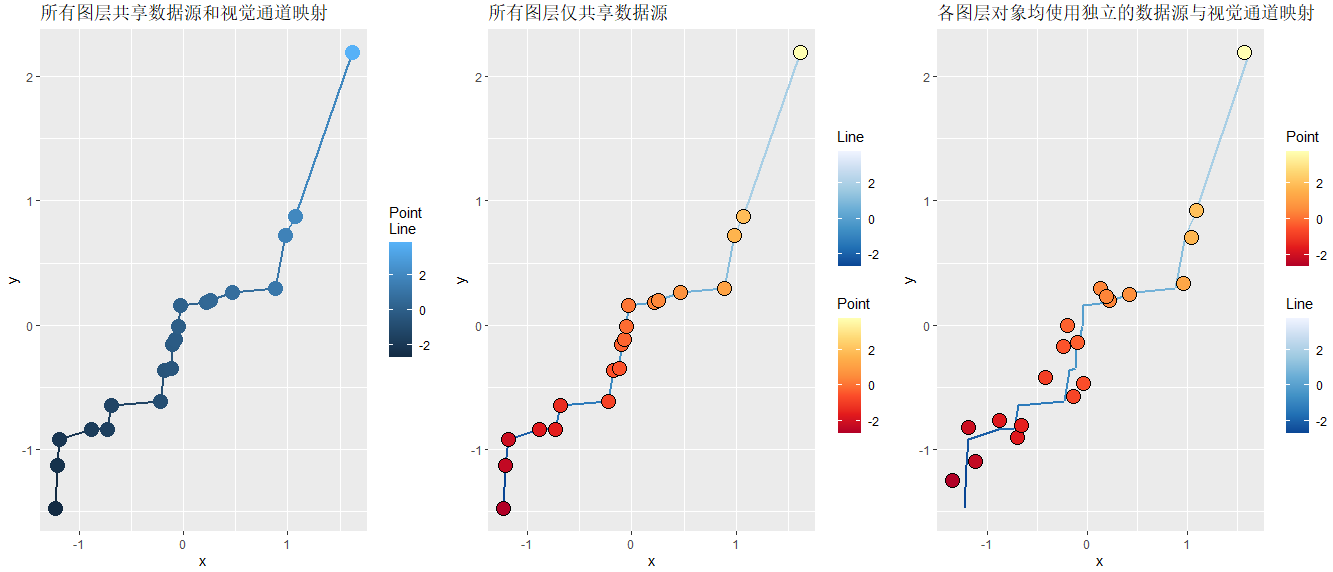
\includegraphics[width=\textwidth]{screenshot044}
\end{figure}
\section{连续型颜色主题方案}
\begin{lstlisting}[language=r]
#EasyCharts团队出品,
#如有问题修正与深入学习,可联系微信:EasyCharts

library(ggplot2)
setwd("E:/11.R/R语言数据可视化之美/Beautiful-Visualization-with-R-master/第1章 R语言编程与绘图基础")
df<-read.csv("Facet_Data.csv", header = TRUE)


library(RColorBrewer)

p1 <- ggplot(df, aes(x=SOD,y=tau,fill=Class)) + 
geom_point(shape=21,size=3,colour="black",stroke=0.25) +
scale_fill_brewer(palette='Set1')+
theme(
text=element_text(size=14,color="black"),
plot.title=element_text(size=14,family="myfont",face="bold.italic",hjust=.5,color="black"),
legend.background = element_blank(),
legend.position=c(0.8,0.15)
)

library(viridis)
p2 <- ggplot(df, aes(x=SOD,y=tau,fill=Class)) + 
geom_point(shape=21,size=3,colour="black",stroke=0.25) +
scale_fill_viridis(option = "plasma",discrete =TRUE)+
theme(
text=element_text(size=14,color="black"),
plot.title=element_text(size=14,family="myfont",face="bold.italic",hjust=.5,color="black"),
legend.background = element_blank(),
legend.position=c(0.8,0.15)
)


library(wesanderson)
p3 <- ggplot(df, aes(x=SOD,y=tau,fill=Class)) + 
geom_point(shape=21,size=3,colour="black",stroke=0.25) +
scale_fill_manual(values=wes_palette("Darjeeling1")[c(1,3,5)])+
theme(
text=element_text(size=14,color="black"),
plot.title=element_text(size=14,family="myfont",face="bold.italic",hjust=.5,color="black"),
legend.background = element_blank(),
legend.position=c(0.8,0.15)
)


p4 <- ggplot(df, aes(x=SOD,y=tau,fill=Class)) + 
geom_point(shape=21,size=3,colour="black",stroke=0.25) +
scale_fill_manual(values=c("#E7298A","#66A61E","#E6AB02"))+
theme(
legend.background = element_blank(),
legend.position=c(0.8,0.15)
)


p5 <- ggplot(df, aes(x = tau, y = SOD, fill=age)) +
geom_point(shape=21,size=4,colour="black",alpha=0.95) +
scale_fill_distiller(palette="RdYlBu")+
theme(
text=element_text(size=15,color="black"),
plot.title=element_text(size=15,family="myfont",face="bold.italic",hjust=.5,color="black"),
legend.background = element_blank(),
legend.position=c(0.85,0.2)
)


p6 <- ggplot(df, aes(x = tau, y = SOD, fill=age)) +
geom_point(shape=21,size=4,colour="black",alpha=0.95) +
scale_fill_viridis(option = "viridis",discrete =FALSE)+
theme(
text=element_text(size=15,color="black"),
plot.title=element_text(size=15,family="myfont",face="bold.italic",hjust=.5,color="black"),
legend.background = element_blank(),
legend.position=c(0.85,0.2)
)

p7 <- ggplot(df, aes(x = tau, y = SOD, fill=age)) +
geom_point(shape=21,size=4,colour="black",alpha=0.95) +
scale_fill_gradient2(low="#00A08A",mid="white",high="#FF0000",midpoint = mean(df$age))+
theme(
text=element_text(size=15,color="black"),
plot.title=element_text(size=15,family="myfont",face="bold.italic",hjust=.5,color="black"),
legend.background = element_blank(),
legend.position=c(0.85,0.2)
)

p8 <- ggplot(df, aes(x = tau, y = SOD, fill=age)) +
geom_point(shape=21,size=4,colour="black",alpha=0.95) +
scale_fill_gradientn(colors= terrain.colors(10))+
theme(
text=element_text(size=15,color="black"),
plot.title=element_text(size=15,family="myfont",face="bold.italic",hjust=.5,color="black"),
legend.background = element_blank(),
legend.position=c(0.85,0.2)
)

library(gridExtra)
grid.arrange(p1,p2,p3,p4,p5,p6,p7,p8,ncol=4,nrow=2)
\end{lstlisting}
\begin{figure}[H]
	\centering
	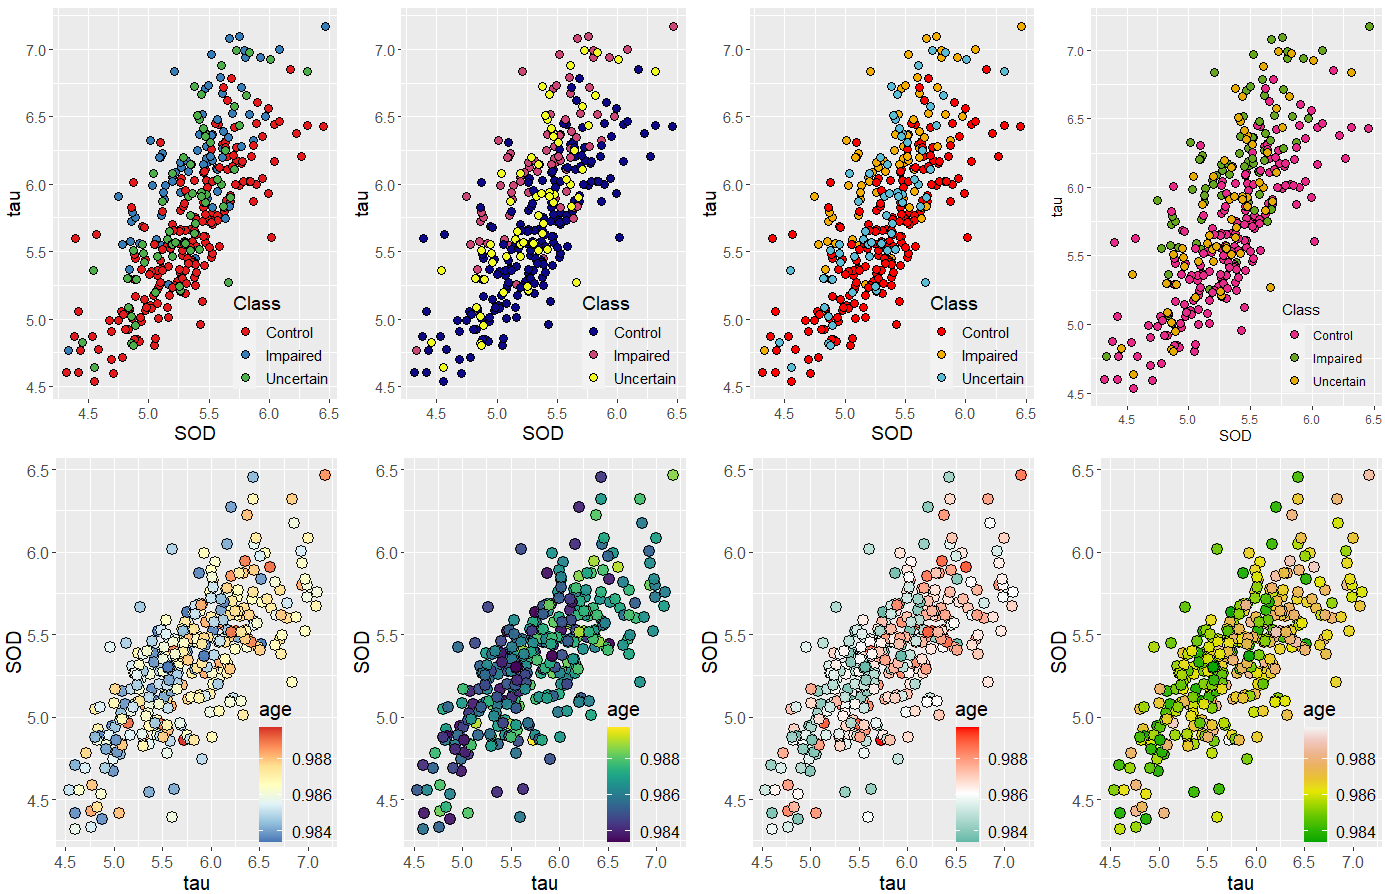
\includegraphics[width=\textwidth]{screenshot045}
\end{figure}
\section{相关系数图}
\begin{lstlisting}[language=r]
library(ggplot2)  
library(RColorBrewer)  
library(reshape2) 

mat <- round(cor(mtcars), 1)
mydata <- melt(mat)  
colnames(mydata)<-c("Var1","Var2","value")

mydata$AbsValue<-abs(mydata$value)

#(b) 双色渐变系颜色方案---------------------------------------------------------
ggplot(mydata, aes(x= Var1 , y=Var2)) +
geom_point(aes(size=AbsValue,fill = value), shape=21, colour="black") +
scale_fill_gradientn(colours=c(brewer.pal(7,"Set1")[2],"white",brewer.pal(7,"Set1")[1]),na.value=NA)+
scale_size_area(max_size=12, guide=FALSE) +
theme(
text=element_text(size=15,face="plain",color="black"),
axis.title=element_text(size=13,face="plain",color="black"),
axis.text = element_text(size=12,face="plain",color="black"),
legend.position="right"
)
# R多色系颜色方案---------------------------------------------------------
mydata$Ceilingcound<-ceiling(mydata$value)

ggplot(mydata, aes(x= Var1 , y=Var2)) +
geom_point(aes(size=AbsValue,fill  = factor(Ceilingcound)), shape=21, colour="black") +
scale_fill_manual(values =c(brewer.pal(7,"Set1")[2],brewer.pal(7,"Set1")[1]),labels=c('Negative','Positive'),na.value=NA,name="factor")+
scale_size_area(max_size=12, guide=FALSE) 

\end{lstlisting}
\begin{figure}[H]
	\centering
	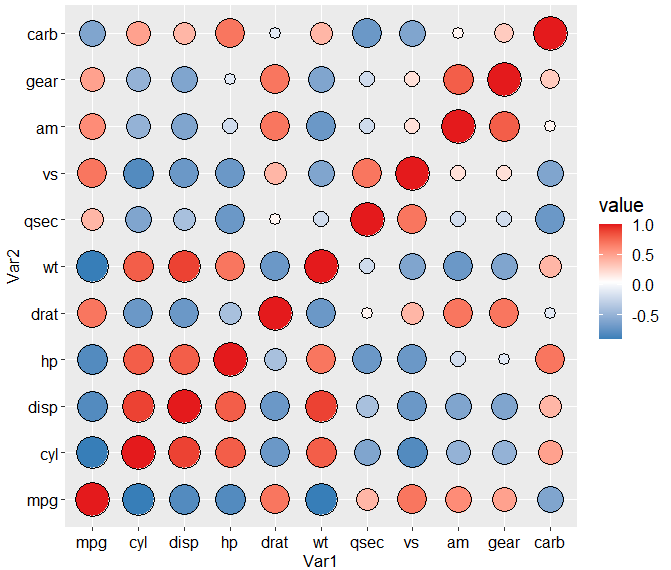
\includegraphics[width=0.5\textwidth]{screenshot046}
\end{figure}
\begin{figure}[H]
	\centering
	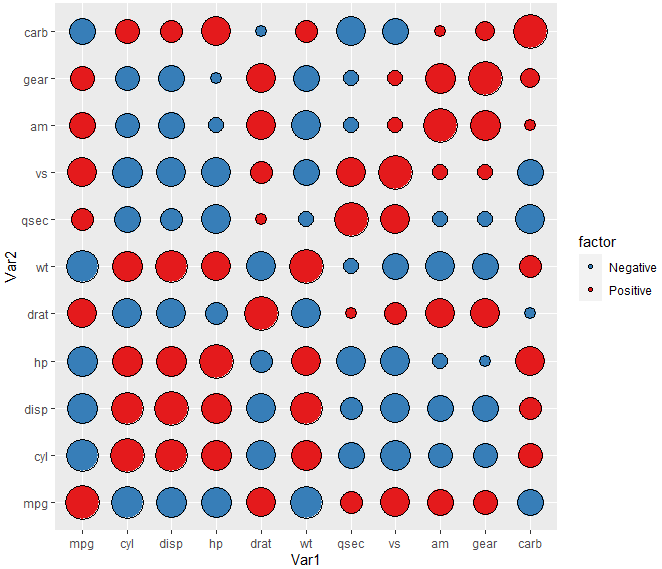
\includegraphics[width=0.5\textwidth]{screenshot047}
\end{figure}
\section{时间序列柱形图}
\begin{lstlisting}[language=r]
library(ggplot2)
library(RColorBrewer)

mydata<-read.csv("Column_Data.csv",stringsAsFactors=FALSE)
mydata$Date<-as.Date(mydata$Date)

ggplot(data = mydata, aes(x = Date, y = temperature,fill = temperature)) +
geom_bar(stat = "identity", width = 2)+
scale_fill_gradient2("Temperature",low=brewer.pal(7,"Set1")[2],mid="grey90",high=brewer.pal(7,"Set1")[1],midpoint=0)+
scale_y_continuous(name="Temperature", limits=c(-10, 30))+
theme(
panel.background=element_rect(fill="white",colour="black"),
panel.grid.major = element_line(colour = "grey60",size=.25,linetype ="dotted" ),
panel.grid.minor = element_line(colour = "grey60",size=.25,linetype ="dotted" ),

axis.title=element_text(size=15),
axis.text.x = element_text(color="black",size=12),
axis.text.y = element_text(color="black",size=12),

legend.text=element_text(size=10),
legend.title=element_text(color="black",size=12),
legend.title.align = 0.5,
legend.position=c(0.15,0.75))
\end{lstlisting}
\begin{figure}[H]
	\centering
	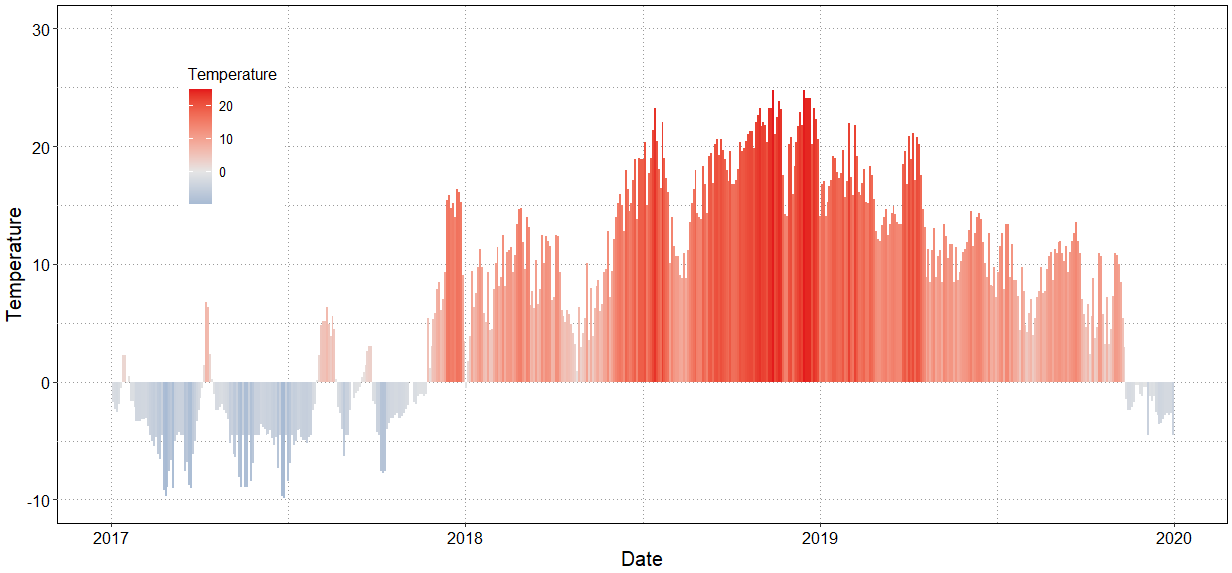
\includegraphics[width=\textwidth]{screenshot048}
\end{figure}
\begin{lstlisting}[language=r]
library(ggplot2)
library(RColorBrewer)
library(Cairo)
library(showtext)


mydata<- read.csv("Bar_Data.csv",stringsAsFactors=FALSE)

mydata$Team<-as.character(mydata$Team)


mydata<-transform(mydata, label1=ifelse(Difference>=0, Team, NA),
label2=ifelse(Difference>0, NA,Team))


mydata$Team <- factor(mydata$Team, levels = mydata$Team[order(mydata$Difference)])

#CairoPDF(file="图1-8-15(a)_条形图.pdf",width=5.28,height=5.47) 
#showtext.begin()
ggplot(data = mydata, aes(x = Team, y = Difference,fill = Difference)) +
geom_bar(stat = "identity", width = 0.8,colour="black",size=0.25)+
scale_fill_gradient2(low=brewer.pal(7,"Set1")[2],mid="grey90",high=brewer.pal(7,"Set1")[1],midpoint=0)+
geom_text(aes(y = 0,     label=label2),size=3,hjust=-0.1)+ #添加负值部分的数据标签
geom_text(aes(y = -0.001,label=label1),size=3,hjust= 1.1)+ #添加正值部分的数据标签
coord_flip() +   #坐标轴翻转
ylim(-5,5)+
theme_minimal() + #图表主题设定
theme(
panel.grid.major=element_blank(),
panel.grid.minor=element_blank(),
panel.grid.major.x = element_line(colour = "grey80",size=.25),
panel.grid.minor.x = element_line(colour = "grey80",size=.25),
plot.title=element_text(size=15,hjust=.5),
axis.text.x = element_text(face="plain", color="black",
size=11, angle=0),
axis.text.y = element_blank(),
legend.position="right",
legend.text=element_text(size=10),
legend.title=element_text(size=10))
#showtext.end()
#dev.off()
\end{lstlisting}
\begin{figure}[H]
	\centering
	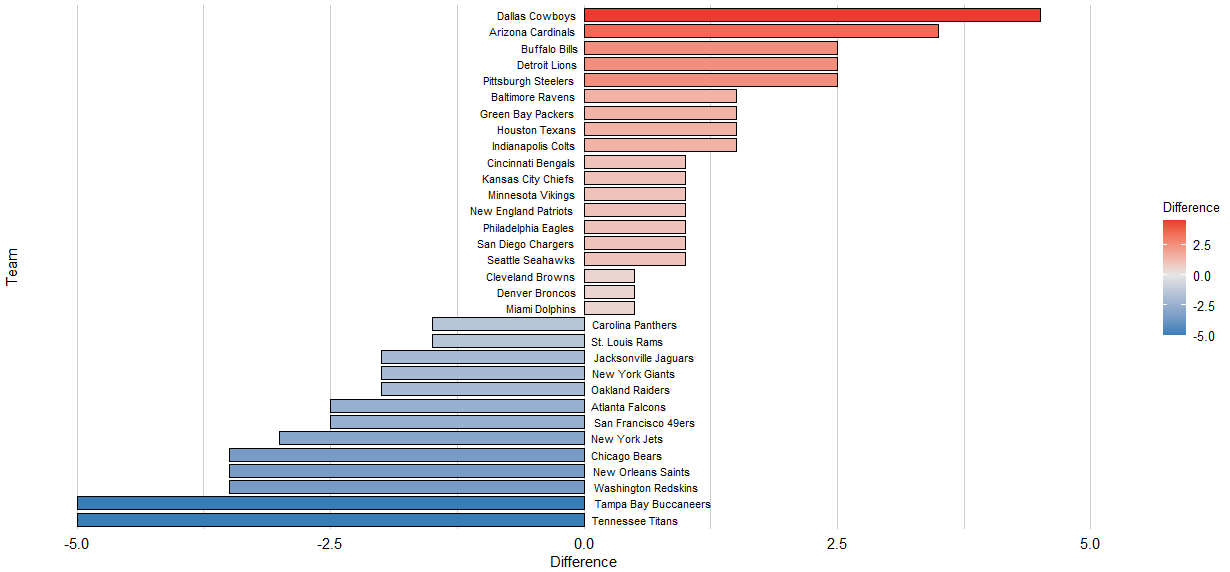
\includegraphics[width=\textwidth]{screenshot049}
\end{figure}

\chapter{R语言数据处理基础}
1.dplyr包:变量筛选函数select(), 记录筛选函数filter(), 排序函数arrange(), 变形(计算)函数mutate(), 汇总函数summarize(), 分组函数group $ \_ $by(),随机抽样函数sample$ \_ $n(),sample$ \_ $frac(),以及多部操作连接符$ \%>\% $...

2.tidyr包: 在具体应用中,tidyr经常与dplyr共同使用. gather()函数用于将款数据转换为长数据; spread()函数用于将长数据转换为宽数据; unite()函数将多列数据合并为一列数据; separate()函数用于将一列数据分离为多列数.

3.reshape2包: 用于数据重构. melt(),cast()实现了长数据和宽数据之间的转换...

4.tidyverse包: 同时调出八个包:ggplot2, dplyr, tidyr, readr, purrr, tibble, stringr, forcats. 

\section{表格的转换}
\subsection{表格的变换}

\begin{lstlisting}[language=r]
> df <- data.frame(x=c("A","B","C"),'2010'=c(1,3,4),'2011'=c(3,5,2),check.names = FALSE)
> df
x 2010 2011
1 A    1    3
2 B    3    5
3 C    4    2
\end{lstlisting}

(1)将宽数据转换为长数据
\begin{lstlisting}[language=r]
> df_melt <- reshape2::melt(df,id.vars="x",variable.name="year",value.name="value")
> df_melt
x year value
1 A 2010     1
2 B 2010     3
3 C 2010     4
4 A 2011     3
5 B 2011     5
6 C 2011     2
> df_gather <- tidyr::gather(df,year,value,-x)
> df_gather
x year value
1 A 2010     1
2 B 2010     3
3 C 2010     4
4 A 2011     3
5 B 2011     5
6 C 2011     2
\end{lstlisting}

id.vars("x")表示由标识变量构成的向量,用于表示观测的变量;

variable.name("year")表示用于保存原始变量名的变量的名称;

value.name("value")表示用于保存原始值的名称.

(2)将长数据转换为宽数据
\begin{lstlisting}[language=r]
> df_dcast <- reshape2::dcast(df_melt,x~year,value.var="value")
> df_dcast
  x 2010 2011
1 A    1    3
2 B    3    5
3 C    4    2

> df_spread <- tidyr::spread(df_gather,year,value)
> df_spread
  x 2010 2011
1 A    1    3
2 B    3    5
3 C    4    2
\end{lstlisting}

\subsection{变量的变换}

R内置函数transform()为元数据框添加新的列,可以改变原变量列的值,也可以赋值NULL删除列变量.
\begin{lstlisting}[language=r]
> dat1 <- transform(df_melt,value2=value*2)
> dat1
x year value value2
1 A 2010     1      2
2 B 2010     3      6
3 C 2010     4      8
4 A 2011     3      6
5 B 2011     5     10
6 C 2011     2      4
\end{lstlisting}

我们也可以结合向量化的条件语句ifelse()进行复杂的运算.
\begin{lstlisting}[language=r]
	
\end{lstlisting}
\begin{lstlisting}[language=r]
	
\end{lstlisting}

\end{document}